\documentclass[nobib]{tufte-handout}


\usepackage{ifluatex, ifxetex} % проверка, как компилируется файл

% black magic!
% solving problem with tufte-handout + xelatex
% http://tex.stackexchange.com/questions/200722/
% https://tex.stackexchange.com/questions/47576/
\ifx\ifxetex\ifluatex\else % если xelatex или lualatex
  \newcommand{\textls}[2][5]{%
    \begingroup\addfontfeatures{LetterSpace=#1}#2\endgroup
  }
  \renewcommand{\allcapsspacing}[1]{\textls[15]{#1}}
  \renewcommand{\smallcapsspacing}[1]{\textls[10]{#1}}
  \renewcommand{\allcaps}[1]{\textls[15]{\MakeTextUppercase{#1}}}
  \renewcommand{\smallcaps}[1]{\smallcapsspacing{\scshape\MakeTextLowercase{#1}}}
  \renewcommand{\textsc}[1]{\smallcapsspacing{\textsmallcaps{#1}}}
\fi

% с альтернативного источника:
%\ifluatex % Allow rendering with LuaTeX by setting up the spacing using fontspec features
%  \renewcommand\allcapsspacing[1]{{\addfontfeature{LetterSpace=15}#1}}
%  \renewcommand\smallcapsspacing[1]{{\addfontfeature{LetterSpace=10}#1}}
%\fi

% lua produces strange notes
% https://tex.stackexchange.com/questions/328431

\usepackage{fontspec} % работа со шрифтами
\usepackage{polyglossia} % учим русский как иностранный :)

\setmainlanguage{russian}
\setotherlanguages{english}

% заменяем --- на тире, << на кавычки и т.д.:
\defaultfontfeatures{Ligatures = TeX}

% download "Linux Libertine" fonts:
% http://www.linuxlibertine.org/index.php?id=91&L=1
\setmainfont{Linux Libertine O} % or Helvetica, Arial, Cambria
% why do we need \newfontfamily:
% http://tex.stackexchange.com/questions/91507/
\newfontfamily{\cyrillicfonttt}{Linux Libertine O}
\newfontfamily{\cyrillicfont}{Linux Libertine O}
\newfontfamily{\cyrillicfontsf}{Linux Libertine O}



\usepackage{amsmath}
\usepackage{amsthm}
\usepackage{amsfonts}
\usepackage{amssymb}
\usepackage{url} % вставка \url{}
\usepackage{graphicx} % вставка графиков
\usepackage{csquotes} % адаптирующиеся кавычки командой \enquote{}
\usepackage{comment} % ingore everything between \begin{comment} \end{comment}
\usepackage{answers} % separate problems and solutions
\usepackage{tikz} % pictures with tikz language
\usepackage{todonotes} % todo in documents


\usepackage{enumitem} % для создания своих нумерующих списков (хак для гиперссылок)

%\usepackage[left=2cm,right=2cm,top=2cm,bottom=2cm]{geometry}

\theoremstyle{definition}
% \newtheorem{problem}{Задача}
% \numberwithin{problem}{section}

\Newassociation{sol}{solution}{solution_file}
% sol — имя окружения внутри задач
% solution — имя окружения внутри solution_file
% solution_file — имя файла в который будет идти запись решений
% можно изменить далее по ходу


% very useful during de-bugging!
% \usepackage[left]{showlabels}
% \showlabels{hypertarget}
% \showlabels{hyperlink}

% магия для автоматических гиперссылок задача-решение
\newlist{myenum}{enumerate}{3}
% \newcounter{problem}[chapter] % нумерация задач внутри глав
\newcounter{problem}

\newenvironment{problem}%
{%
\refstepcounter{problem}%
%  hyperlink to solution
     % \hypertarget{problem:{\thechapter.\theproblem}}{} % нумерация внутри глав
     \hypertarget{problem:{\theproblem}}{}
     %\Writetofile{solution_file}{\protect\hypertarget{soln:\thechapter.\theproblem}{}}
     \Writetofile{solution_file}{\protect\hypertarget{soln:\theproblem}{}}
     % \begin{myenum}[label=\bfseries\protect\hyperlink{soln:\thechapter.\theproblem}{\thechapter.\theproblem},ref=\thechapter.\theproblem]
     \begin{myenum}[label=\bfseries\protect\hyperlink{soln:\theproblem}{\theproblem},ref=\theproblem]
     \item%
    }%
    {%
    \end{myenum}}
% для гиперссылок обратно надо переопределять окружение
% это происходит непосредственно перед подключением файла с решениями


\DeclareMathOperator{\Var}{Var}
\DeclareMathOperator{\card}{card}
\DeclareMathOperator{\Cov}{Var}
\DeclareMathOperator{\E}{E}
\renewcommand{\P}{\mathbb{P}}
\newcommand{\I}{\mathbb{I}} % индикатор события



\usepackage[bibencoding = auto, backend = biber,
sorting = none]{biblatex}

\addbibresource{probability_dna.bib}





\title{Теория вероятностей: культурный код}
\author{Фольклор}
\date{\today}
\begin{document}



\maketitle

\section{Культурный код}

Сборник восхитительных задач по элементарной теории вероятностей.
Эти задачи — наша вероятностная ДНК.

\section{Фольклор и красота}


\Opensolutionfile{solution_file} % [sols_chap_07]
% в квадратных скобках можно уточнить фактическое имя файла



\begin{problem}
Задача о Сумасшедшей Старушке.

\marginnote{Родилась она чисто из жизни — а именно, тогда,
когда ещё юному автору приходилось часто ездить из Питера во Псков.
Чаще всего билет на покупался в общий вагон поезда. На билете всегда было указано место.
Но не тут-то было! Приходя в вагон, обнаруживалось,
что пришедшие первыми занимали самые лучшие места
(утверждая, что номера мест на билетах — это просто для статистики).
И вот тут-то и начинались эти цепочные сгоняния пассажиров.
В оригинале задачка звучала так:
«В общем вагоне поезда Ленинград-Псков $N$ мест\ldots $N$-й пассажир,
придя последним, обнаруживал,
что свободно только только самое дурацкое место — около туалета\ldots»
Но в редакции Кванта решили, что писать про бардак и туалет в общем вагоне
поезда Лениград-Псков как-то не очень. И самовольно переделали условие на кинотеатр,
\url{http://kvant.mccme.ru/1985/06/p34.htm}, автор: Игорь Алексеев}

В самолёте $100$ мест и все билеты проданы.
Первой в очереди на посадку стоит Сумасшедшая Старушка.
Сумасшедшая Старушка очень переживает, что ей не хватит места,
врывается в самолёт и несмотря на номер по билету садиться на случайно выбираемое место.
Каждый оставшийся пассажир садится на своё место, если оно свободно,
и на случайное выбираемое место, если его место уже кем-то занято.

\begin{enumerate}
% \item Какова вероятность того, что все пассажиры сядут на свои места?
%\item Какова вероятность того, что второй пассажир в очереди сядет на своё место?
\item Какова вероятность того, что последний пассажир сядет на своё место?
\item Чему примерно равно среднее количество пассажиров севших на свои места?
\end{enumerate}

\begin{figure*}
  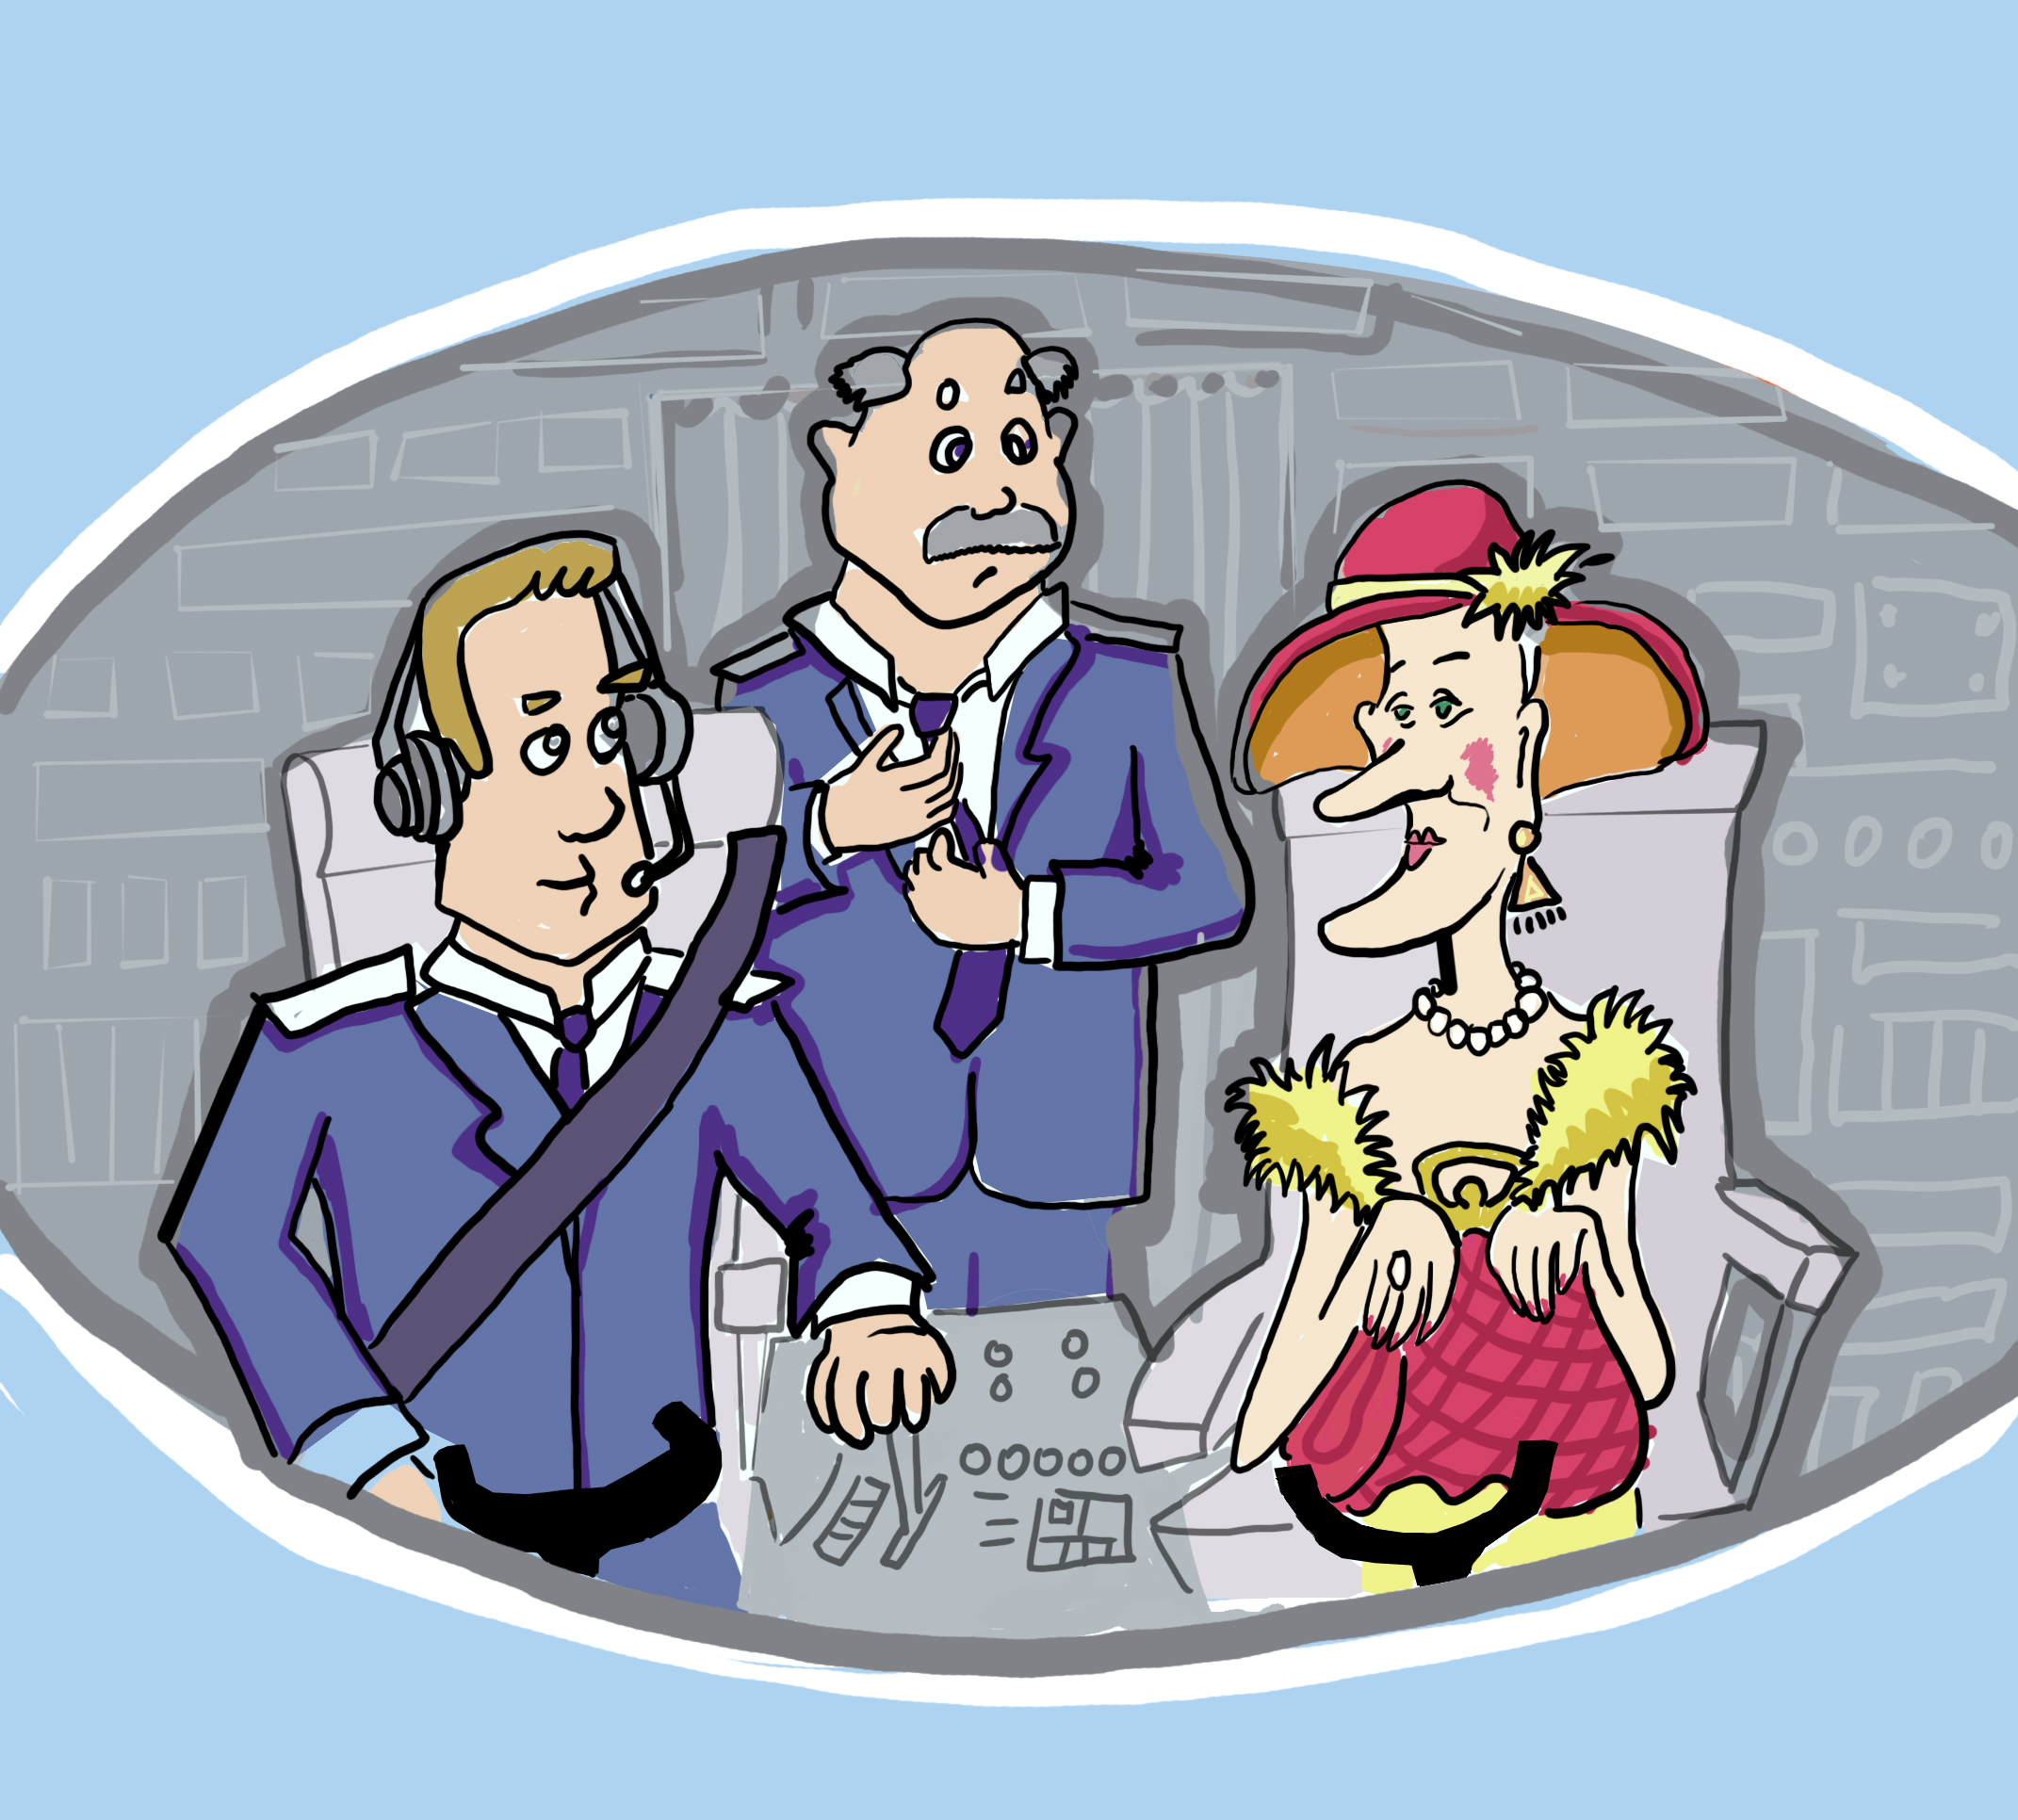
\includegraphics[width=17cm]{images/crazy_woman.jpg}
  \caption{— Простите, пожалуйста, это место 1Б?}
\end{figure*}


\begin{sol}
Решение раз. Рассмотрим последовательность пересаживаний,
начинающуюся с сумасшедшей старушки.
В этой последовательности последний пассажир и
сама сумасшедшая старушка равновероятно опережают друг друга.
Следовательно, искомая вероятность равна $1/2$.

Решение два. Решаем задачу для $n=2$, $n=2$, получаем вероятность $1/2$.
База индукции есть. Предположим, что
для $1$, $2$, \ldots, $n-1$ пассажира вероятность равна $1/2$.
В случае $n$ пассажиров первым ходом старушка может занять своё место,
место последнего, какое-то другое место. Если она заняла своё,
то последний точно сядет на своё место. Если она заняла место последнего,
то он точно не сядет на своё место. Если она сядет на одно из оставшихся мест,
то вскоре очередь дойдёт до того пассажира, чьё место она заняла.
В этот момент можно считать, что он превратится в сумасшедшую старушку.
Для меньшего количество пассажиров задача решена и даёт вероятность $1/2$.
В силу симметрии получаем вероятность $1/2$ и для $n$ пассажиров.
\end{sol}

\end{problem}



\begin{problem}
На самолёт, имеющий $100$ мест, проданы все билеты. Для посадки в
самолёт пассажиры выстроились в очередь. Первые 99 пассажиров — сумасшедшие старушки.
Они садятся на наугад выбранные места. Последний пассажир садится на то место,
которое указано в его билете. Если это место занято, то он с
помощью стюардессы сгоняет старушку со своего законного места.
Согнанная с чужого места сумасшедшая старушка становится
благоразумной и садится на свое место по билету. Возможно для
этого придется согнать еще одну старушку и т.д.
\begin{enumerate}
\item Какова вероятность того, что потревожат старушку, стоявшую $i$-ой в очереди?
\item Каково ожидаемое количество потревоженных старушек?
\end{enumerate}

\begin{sol}
\begin{enumerate}
\item Чтобы потревожили старушку, стоявшую $i$-ой в очереди,
эта старушка должна случайным образом выбрать то место из $101-i$ оставшегося,
которое по билету принадлежит последнему пассажиру,
или же сесть на место другой сумасшедшей старушки так,
чтобы в итоге другая сумасшедшая старушка попросила ее пересесть.

Если старушки случайно выбирают место в порядке очереди,
то $i$-ая старушка будет выбирать $1$ место из $101-i$.
Вероятность случайно выбрать место одинакова для всех мест, а значит:

$\P(\text{i grandma will choose the last passenger`s seat})=1 - \frac{1}{101-i} =
 \frac{100-i}{101-i}$.

НО: здесь еще надо учесть ситуацию, когда в итоге $i$-ая старушка будет потревожена другой.

Ответ: min $\P(\text{i grandma will be bothered}) =\frac{100-i}{101-i}$

\item Одну из старушек потревожат с вероятностью $\frac{1}{100}$,
так как она должна была случайно выбрать одно из $100$ мест.
Если её потревожили, то с вероятностью $\frac{98}{99}$ место, указанное в ее билете,
будет занято, что преполагает пересаживание еще одной старушки и т.д.

Ноль старушек будет потревожено с вероятностью $\frac{99}{100}$,
лишь одна старушка будет потревожена с вероятностью $\frac{1}{100} \cdot \frac{1}{99}$,
две старушки будут потревожены с вероятностью
$\frac{1}{100} \cdot \frac{98}{99} \cdot \frac{1}{98}$ и т.д.
Заметим, что при нахождении математического ожидания
можно будет вынести $\frac{1}{9000}$ за скобку, а в ней останется
сумма чисел  от $1$ до $99$.

$\E(X) = 0 \cdot \frac{99}{100} + 1 \cdot \frac{1}{100} \cdot \frac{1}{99} +
2\cdot \frac{1}{100} \cdot \frac{98}{99} \cdot {1}{98} + \ldots  = 0.489$
\end{enumerate}
\end{sol}

\end{problem}


\begin{problem}
Задача собирателя наклеек. Coupon collector's problem.

Производитель чудо-юдо-йогуртов наклеивает на каждую упаковку одну
из 50 случайно выбираемых наклеек. Покупатель собравший все виды наклеек
получает приз от производителя. Пусть $X$ — это количество упаковок йогурта,
которое нужно купить, чтобы собрать все наклейки.

Найдите  $\E(X)$, $\Var(X)$.

\begin{sol}
Количество наклеек можно разложить в сумму независимых случайных величин,
\[
X=Z_1+Z_2+\ldots+Z_n,
\]
где $Z_i$ — количество наклеек, которые нужно докупить,
чтобы найти $i$-ый новый вид наклейки, когда в коллекции уже есть наклейки $i-1$ вида.
Конечно, $Z_1=1$.

Замечаем, что $\E(Z_i)=\ldots $, $\Var(Z_i)=\ldots $.
\end{sol}

\end{problem}


\begin{problem}
Спички Банаха. Banach's matchbox problem.

Польский математик Стефан Банах имел привычку носить
в каждом из двух карманов пальто по коробку спичек.
Всякий раз, когда ему хотелось закурить трубку,
он выбирал наугад один из коробков и доставал из него спичку.
Первоначально в каждом коробке было по $n$ спичек.
Но когда-то наступает момент, когда выбранный наугад коробок оказывается пустым.

\begin{enumerate}
\item Какова вероятность того,
что в другом коробке в этот момент осталось ровно $k$ спичек?
\item Каково среднее количество спичек в другом коробке?
\end{enumerate}

\begin{sol}
\begin{enumerate}
\item Обозначим оставшееся количество спичек в другом кармане буквой $X$.

Рассмотрим случай, когда Банах обнаруживает пустым правый карман.
Следовательно, Банах проверил оба своих кармана всего $n-k+n=2n-k$ раз,
из которых $n-k$ раз он проверил левый карман, $n$ раз — правый,
а сейчас лезет в правый карман.

Используя формулу для биномиального распределения получаем:
\[
C_{2n-k}^n \left(\frac{1}{2}\right)^{n-k}\cdot
\left(\frac{1}{2}\right)^{n}\cdot \frac{1}{2}=
C_{2n-k}^{n}\left(\frac{1}{2}\right)^{2n-k+1}
\]

Второй случай рассматривается аналогично, если мы просто поменяем карманы местами.
Умножаем полученную вероятность на $2$, получаем:
\[
\P(X=k)=2\cdot C_{2n-k}^{n}\left(\frac{1}{2}\right)^{2n-k+1}=
C_{2n-k}^{n}\left(\frac{1}{2}\right)^{2n-k}
\]
\item
\end{enumerate}
\end{sol}

\end{problem}


\begin{problem}
Равновесие Харди-Вайнберга.

Предположим, что три возможных генотипа \verb|aa|, \verb|Aa| и \verb|AA|
изначально встречаются с частотами $p_1$, $p_2$ и $p_3$, где $p_1+p_2+p_3=1$.
Ген не сцеплен с полом,
поэтому частоты $p_1$, $p_2$ и $p_3$ одинаковы для мужчин и для женщин.
\begin{enumerate}
\item У семейных пар из этой популяции рождаются дети.
Назовём этих детей первым поколением.
Каковы частоты для трёх возможных генотипов в первом поколении?
\item У семейных пар первого поколения тоже рождаются дети.
Назовём этих детей вторым поколением.
Каковы частоты для трёх возможных генотипов во втором поколении?
\item Каковы частоты для трёх возможных генотипов в $n$-ном поколении?
\item Заметив явную особенность предыдущего ответа сформулируйте
теорему о равновесии Харди-Вайнберга.
Прокомментируйте утверждение: «Любой рецессивный ген со временем исчезнет».
\end{enumerate}

\begin{sol}
Рассмотрим все варианты скрещивания и вероятности:

\begin{tabular}{ll}
$\verb|AA|*\verb|AA|$ & $p_1^2$ \\
$\verb|AA|*\verb|Aa|$ & $2 \cdot p_1 \cdot p_2$ \\
$\verb|AA|*\verb|aa|$ & $2 \cdot p_1 \cdot p_3$ \\
$\verb|Aa|*\verb|Aa|$ & $p_2^2$ \\
$\verb|Aa|*\verb|aa|$ & $2\cdot p_2 \cdot p_3$ \\
$\verb|aa|*\verb|aa|$ & $p_3^3$
\end{tabular}

Зная, какие дети рождаются у всевозможных пар,
составим аналогичную таблицу вероятностей для генотипов детей (свернув далее в квадраты):

\begin{tabular}{ll}
$\verb|AA|$ & $p_1^2+p_1 \cdot p_2+0.25 \cdot p_2^2 = p^2$ \\
$\verb|Aa|$ & $p_1 \cdot p_2+p_2 \cdot p_3+0.5 \cdot p_2^2+2 \cdot p_1 \cdot p_3 = 2pq$ \\
$\verb|aa|$ & $p_3^2+p_2 \cdot p_3+0.25 \cdot p_2^2 = q^2$
\end{tabular}

Видим, что всё это сворачивается в полные квадраты:

$\verb|AA|: (p_1+0.5 \cdot p_2)^2 = p'^2$

$\verb|Aa|: 2(p_1+0.5 \cdot p_2)^2\cdot (p_3+0.5 \cdot p_2)^2 = 2p'q'$

$\verb|aa|:(p_3+0.5 \cdot p_2)^2 = q'^2$

Соотношение генов не изменилось и всё ещё удовлетворяет уравнению $p'^2+2p'q'+q'^2=1$

Потому соотношение генов в любом поколении не меняется,
а значит, рецессивный ген со временем не исчезает.
\end{sol}

\end{problem}


\begin{problem}
Поляризация света.

Световая волна может быть разложена на две поляризованные составляющие,
вертикальную и горизонтальную.
Поэтому состояние отдельного поляризованного фотона
может быть описано углом $\alpha$.
\marginnote{На самом деле внутренний мир фотона гораздо разнообразнее.}
Поляризационный фильтр описывается углом поворота $\theta$.
Фотон в состоянии $\alpha$ задерживается поляризационным фильтром с параметром $\theta$
с вероятностью $p=\sin^2(\alpha-\theta)$ или проходит сквозь фильтр с вероятностью $1-p$,
переходя при этом в состояние $\theta$.

\begin{enumerate}
\item Какова вероятность того,
что поляризованный фотон в состоянии $\alpha$ пройдёт сквозь фильтр с параметром $\theta=0$?
\item Имеется два фильтра и поляризованный фотон в состоянии $\alpha$.
Первый фильтр — с $\theta=0$, второй — c $\theta=\pi/2$.
Какова вероятность того, что фотон пройдет через оба фильтра?
\item Имеется три фильтра и поляризованный фотон в состоянии $\alpha$.
Первый фильтр — с $\theta=0$, второй — c $\theta=\beta$, третий — с $\theta=\pi/2$.
Какова вероятность того, что фотон пройдет через все три фильтра?
При каких $\alpha$ и $\beta$ она будет максимальной и чему при этом она будет равна?
\marginnote{Как сделать «секретный монитор» своими руками,
\url{http://www.youtube.com/watch?v=-ojbykV1zyc}}
\item Объясните следующий фокус. Фокусник берет два специальных стекла и видно,
что свет сквозь них не проходит. Фокусник ставит между двумя стёклами третье,
и свет начинает проходить через три стекла.
\end{enumerate}

\begin{sol}
\begin{figure*}
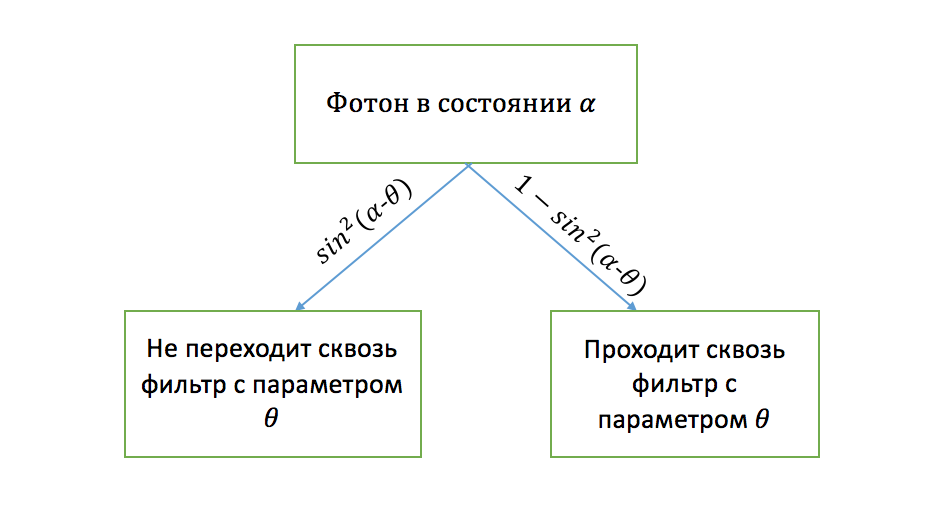
\includegraphics[width=10cm]{images/tree_task6.jpg}
\end{figure*}
\begin{enumerate}
\item $\P(\text{фотон в состоянии } \alpha
\text{ пройдет через фильтр с параметром } \theta = 0)
= 1 - \sin^2(\alpha-0) = \cos^2(\alpha)$
\item $\P(\text{фотон пройдет сквозь фильтр с параметром } \theta = 0
\text{, переходя в состояние} 0) = 1 - \sin^2(\alpha) = \cos^2(\alpha)$

$\P(\text{фотон в состоянии } 0
\text{ пройдёт сквозь фильтр с параметром } \theta = \pi/2)
=   1−\sin^2(0-\pi/2) = \cos^2(-\pi/2)$

Ответ: $\P(\text{фотон в состоянии } \alpha
\text{ пройдет через фильтр с параметром } \theta = 0
\text{ и сквозь второй фильтр }  \theta = \pi/2) =
\cos^2(\alpha) \cdot \cos^2(−\pi/2) = 0$
\item $\P(\text{фотон проходит сквозь фильтр с параметром } \theta = 0
\text{, переходя в состояние } 0) = 1 - \sin^2(\alpha) = \cos^2(\alpha)$

$\P(\text{фотон в состоянии } 0
\text{ проходит сквозь фильтр с параметром } \theta = \beta
\text{, переходя в состояние } \beta) =   1−\sin^2(0-\beta) = \cos^2(-\beta)$

$\P(\text{фотон в состоянии } \beta
\text{ проходит сквозь фильтр с параметром } \theta = \pi/2)
=   1−\sin^2(\beta-\pi/2) = \cos^2(\beta-\pi/2)$

Вероятность того, что фотон пройдет поочереди по всем трём фильтрам равна:
$\P =\cos^2(\alpha)\cdot \cos^2(-\beta)\cdot\cos^2(\beta-\pi/2)$

Максимизируя вероятность, получаем $\alpha = \pi/2, \beta = \pi/4$.
При этих значениях $\P = 1/4$.
\item Данный фокус объясняется с помощью уже решенных пунктов 2 и 3.

В пункте 2 мы доказали,что при любых $\alpha$ вероятность того,
что свет сначала пройдет сквозь фильтр с параметром $\theta = 0$,
а потом сквозь фильтр с параметром $\theta=\pi/2$ равняется $0$.
В пункте 3 мы доказали, что если $\alpha = \pi/2$
и между этими фильтрами ставить другой фильтр с параметром $\beta=\pi/4$,
то всегда будет существовать вероятность ($1/4$),
что свет пройдет сквозь 3 фильтра/стекла.
Именно этим и объясняется почему свет не проходит сквозь два стекла,
а когда между ними ставишь другое стекло, то он начинает проходить сквозь три стекла.
\end{enumerate}
\end{sol}

\end{problem}


\begin{problem}
Истеричная певица

Начинающая певица дает концерты каждый день.
Каждый ее концерт приносит продюсеру 0.75 тысяч евро.
После каждого концерта певица может впасть в депрессию с вероятностью 0.5.
Самостоятельно выйти из депрессии певица не может.
В депрессии она не в состоянии проводить концерты.
Помочь ей могут только цветы от продюсера.
Если подарить цветы на сумму $0\le x\le 1$ тысяч евро,
то она выйдет из депрессии с вероятностью $\sqrt{x}$.

Какова оптимальная стратегия продюсера?
Продюсер максимизирует текущую ожидаемую ценность певицы.

\begin{sol}
Рассмотрим совершенно конкурентный невольничий рынок начинающих певиц.
Певицы в хорошем настроении продаются по $V_1$, в депрессии — по $V_2$.
Получаем систему уравнений:
\[
\begin{cases}
  V_1 = 0.75 + (0.5 V_1 + 0.5 V_2) \\
  V_2 = \max_x \sqrt{x}V_1 + (1 - \sqrt{x})V_2 - x
\end{cases}
\]
Оптимизируем и получаем, $x^* = (V_1 - V_2)^2/4$.
Из первого уравнения находим $(V_1 - V_2)/2=0.75$.
\end{sol}

\end{problem}


\begin{problem}
Парадокс Симпсона.  Simpson's Paradox.

Два лекарства испытывали на мужчинах и женщинах. Каждый
человек принимал только одно лекарство. Общий процент людей,
почувствовавших улучшение, больше среди принимавших лекарство А.
Процент мужчин, почувствовавших улучшение, больше среди мужчин, принимавших лекарство В.
Процент женщин, почувствовавших улучшение, больше среди женщин, принимавших лекарство В.

\begin{enumerate}
\item Возможно ли это?
\item Какое лекарство нужно посоветовать принять пациенту, если его пол неизвестен?
\end{enumerate}

\begin{sol}
  Да, возможно.
  \todo[inline]{две иллюстрации: с мозаичными графиками и векторами из Вильямса}
  Если пол неизвестен, то лучше принимать $B$.
\end{sol}

\end{problem}


\begin{problem}
Вовочку перевели из класса А в класс Б.
Мог ли при этом возрасти средний балл по математике в обоих классах?

\begin{sol}
Да, возможно, если уровень Вовочки ниже среднего уровня класса А,
но выше среднего уровня класса Б.
\end{sol}

\begin{figure*}
  
\includegraphics[width=17cm]{images/average.png}
  \caption{Dilbert}
\end{figure*}



\end{problem}


\begin{problem}
Злобный дракон поймал трех гномов. И решил поиграться с ними.
Каждому гному он надевает с равными вероятностями черный или белый колпак.
\marginnote{ — Значит, дракон — это датчик случайных колпаков?}


Гномы видят чужие колпаки, но не видят своих и не могут общаться после выдачи колпаков.
Каждый гном может попытаться угадать цвет своего колпака, либо промолчать.
Дракон отпустит гномов, если хотя бы один гном угадал цвет своего колпака,
и никто не сделал ошибки. Если все одновременно промолчали, или кто-нибудь ошибся,
то все гномы будут съедены. Перед игрой гномы могут договориться о стратегии игры.

\begin{enumerate}
\item Как гномам следует играть, если Злобный дракон спрашивает их по очереди?
Какова вероятность того, что они будут спасены?
\item Как гномам следует играть, если они должны дать ответ одновременно?
Какова вероятность того, что они будут спасены?
\item Если от далекого спутника нужно получить один бит информации («да» или «нет»),
то, отправив три бита, можно не бояться того, что природа «испортит» один из них.
Постройте этот простой код. Проведите аналогию с предыдущим пунктом.
\marginnote{ — Три гнома — три бита?}
\end{enumerate}
Идея этой задачи используется не только при космической связи.
Чтобы неглубокие царапины на компакт диске не вызывали потерь данных,
при записи используется код Рида-Соломона.
\marginnote{ — А как звали третьего гнома?}

\begin{sol}
\begin{enumerate}
\item Присвоим белому колпаку значение $0$, а черному $1$. Первый гном смотрит
на двух остальных и считает «сумму» их колпаков. Пусть по договоренности,
если сумма четная, то гном произносит «белый», нечетная – «чёрный».
Дракон воспринимает высказанное как догадку о цвете колпака первого гнома,
хотя по сути оно таковым не является. У гнома нет данных,
чтобы сделать вывод о цвете своего колпака. С вероятностью 0.5 гном
либо угадал цвет своего колпака, сообщая сумму двум другим игрокам,
и игра продолжается, либо не угадал и все будут съедены.
Допустим, первый считает сумму, видит, что она нечетная, говорит дракону,
что его колпак черный и случайным образом угадывает цвет своего колпака.

Второй, зная сумму, которую назвал первый, смотрит на шапку третьего гнома
и сравнивает «значение» колпака третьего гнома с названной ранее суммой.
Если она не изменилась, то его колпак, очевидно, белый. Изменилась – чёрный.
Из предположения второго третий наверняка знает, какого цвета на нём колпак.

Таким образом, вероятность выигрыша сводится к вероятности того,
что названная первым гномом «сумма» в действительности соответствует цвету его колпака.

\item Итак, у нас есть счётное число гномов, которые увидели дракона.
Эти гномы знают, что колпаки бывают двух цветов — чёрного и белого,
поэтому последовательность из белых и чёрных колпаков
(надетых на головы бедных гномов, конечно)
является последовательностью абсолютно эквивалентной последовательности из нулей и единиц,
рассмотренной в предыдущем пункте.
Что же мешает нам посоветовать гномам заранее определить
представительскую последовательность в каждом классе похожих
(главную звезду в созвездии похожих звёзд колпаков) и угадывать свой цвет, согласно ей?!
Тогда каждый гном, видя цвета колпаков своих друзей, стоящих впереди,
сможет определить класс, к которому принадлежит реальная последовательность колпаков
(определенная драконом при раздаче колпаков).
Так как эта последовательность «похожа» на выбранную гномами в качестве представительской,
то она будет отличаться от нее на конечное число колпаков.
Значит, гадая согласно выбранной последовательности,
лишь конечное число гномов назовут свои цвета неправильно.
\end{enumerate}

\end{sol}

\end{problem}


\begin{problem}
Париж, Людовик XIV, 1654 год, высшее общество говорит о рождении новой науки —
теории вероятностей. Ах, кавалер де Мере,
«fort honnête homme sans être mathématicien»\ldots
\marginnote{«благородный человек, хотя и не математик».}
Старая задача, неправильные решения которой предлагались тысячелетиями
(например, одно из неправильных решений предлагал изобретатель двойной записи,
кумир бухгалтеров, Лука Пачоли) наконец решена правильно!


Два игрока играют в честную игру до шести побед. Игрок первым выигравший шесть партий
(не обязательно подряд) получает 800 луидоров.
К текущему моменту первый игрок выиграл пять партий, а второй — три партии.
Они вынуждены прервать игру в данной ситуации.


Как им поделить приз по справедливости?

\begin{center}
\begin{figure*}[t]
  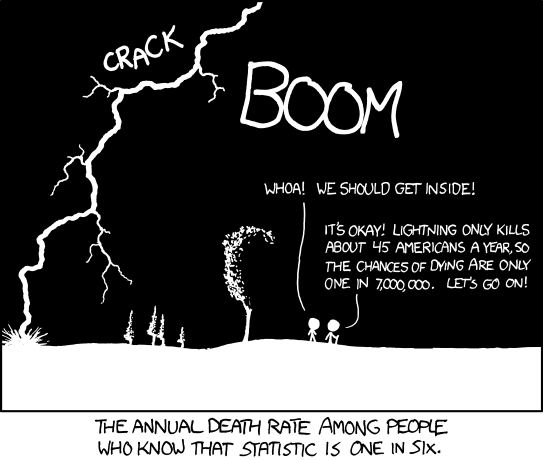
\includegraphics[width=10cm]{images/conditional.png}
  \caption{\url{http://xkcd.com/795/}}
\end{figure*}
\end{center}


\begin{sol}
Проведём ещё 3 партии. Первый игрок проиграет только,
если все три выиграны вторым игроком, то есть с вероятностью $1/8$.
Стало быть $800$ луидоров надо поделить на $100$ и $700$.
\end{sol}

\end{problem}


\begin{problem}
На арене две команды гладиаторов, $A$ и $B$. Каждый гладиатор обладает
определенной силой, неизменной по ходу игры. Команды могут отличаться
по количеству гладиаторов и их силе. Игра проходит в виде последовательных турниров,
в каждом из которых участвует по одному гладиатору от каждой стороны.
Если в очередном турнире встречаются гладиаторы с силами $a$ и $b$,
то вероятность победы первого определяется величиной  $\frac{a}{a+b}$.
Гладиатор, проигравший турнир, выбывает из игры, выигравший — возвращается в команду.
Гладиаторы не устают, но и не приобретают опыта. Стратегия команды предписывает,
какого гладиатора выдвигать на очередной турнир в зависимости текущего состава команд.
Игра ведется до полного выбывания из игры одной из команд.

Как выглядит оптимальная стратегия команды $A$?

\begin{sol}
Для упрощения объяснений временно заменим гладиаторов на лампочки.
У них есть важное свойство: знание о том, сколько времени лампочка уже горит,
не несёт информации о том, сколько она ещё будет гореть.
Единственное распределение с таким свойством — свойством отсутствия памяти — 
экспоненциальное. Если математическое ожидание времени работы лампочки $x$,
то вероятность того, что она всё ещё горит в момент $t$, равна $e^{-t/x}$.

Если взять две лампочки с математическими ожиданиями времени работы,
равными $x$ и $y$ соответственно,
то первая будет гореть дольше второй с вероятностью $\frac{x}{x+y}$.
Встреча двух гладиаторов соответствует «соревнованию» между лампочками:
они горят, пока одна из них не перегорит, а ту, что выиграла,
выключают и могут выбрать для следующего турнира,
причём из-за свойства отсутствия памяти её «сила» в следующем турнире не меняется.

В течение турнира у каждый команды в любой момент времени горит ровно одна лампочка.
Выиграет та, у которой общая длительность горения всех лампочек
(общая сила всех гладиаторов) будет больше.
Поскольку эта общая длительность не зависит от того,
в каком порядке лампочки будут включаться, вероятность того,
что выиграет команда $A$ не зависит от её стратегии.

\end{sol}

\end{problem}


\begin{problem}
В отличие от обычного гладиатора, у победившего гладиатора-вампира сила увеличивается
на силу побежденного им гладиатора-вампира. В остальном правила поединка такие же,
как в предыдущей задаче.

Как выглядит оптимальная стратегия команды $A$?

\begin{sol}
Выпишем суммарную силу каждой из команд: $A = a_1 + \ldots + a_n$ и
$B = b_1 + \ldots + b_m$.

Предположим, что гладиатор из команды $A$ имеет силу $a$
и он побеждает гладиатора из $B$, сила которого была $b$.
В этом случае суммарная сила первой команды увеличивается на $b$,
а суммарная сила второй уменьшается на ту же величину,
так как её гладиатор выбывает из игры.
Однако при этом сила команд $A+B$ остаётся неизменной!
Таким образом, в конце суммарная сила победителя будет $A+B$, а проигравшего – $0$.

Рассчитаем математическое ожидание выигрыша команды $A$ в очередном турнире,
если она выдвинет гладиатора с силой $a$ против гладиатора с силой $b$:

\[
\frac{a}{a+b} \cdot b + \frac{a}{a+b} \cdot (-a) = 0
\]

Поскольку турниры не отличаются друг от друга,
для каждого математическое ожидание будет равно нулю, откуда следует,
что ожидаемый выигрыш команды $A$ равен её начальной суммарной силе.
Пусть $p$ – вероятность того, что выиграет команда $A$,
выпишем математическое ожидание выигрыша команды $A$ во всём турнире:

\[
p \cdot (A+B)+(1-p) \cdot 0=A
\]

Выразив $p = \frac{A}{A+B}$, видим,
что вероятность победы команды $A$ определяется
только соотношением начальных сил обеих команд и не зависит от их стратегий.

Значит, любая стратегия команды $A$ приведёт к одному и тому же результату.
\end{sol}

\end{problem}


\begin{problem}
Маша и Саша играют в быстрые шахматы. У них одинаковый класс игры и
оба предпочитают играть белыми, т.е. вероятность выигрыша белых $p>0.5$.
Партии играются до 10 побед. Первую партию Маша играет белыми.
Она считает, что в следующей партии белыми должен играть тот,
кто выиграл предыдущую партию. Саша считает, что ходить белыми нужно по очереди.
При каком варианте правил у Маши больше шансы выиграть?

\begin{sol}
Максимальное число партий, сыгранное Машей и Сашей = $20$.
В первой партии Маша играет белыми, и выигрывает с вероятностью $p>0.5$.

Независимо от правил Маша может сыграграть максимум $10$ раз, а Саша не больше $9$.
Победитель точно определится за $19$ партий. Победитель – игрок,
выигрывший в большем числе партий,
а значит Машин шанс выиграть не зависит от выбранного варианта правил.
\end{sol}

\end{problem}


\begin{problem}
Гадалка

Маша пишет на бумажках два любых различных натуральных числа по своему выбору.
Одну бумажку она прячет в левую руку, а другую — в правую.
Саша выбирает любую Машину руку. Маша показывает число, написанное на выбранной бумажке.
Саша высказывает свою догадку о том, открыл ли он большее из двух чисел или меньшее.
Если Саша не угадал, то Маша выиграла.

Существует ли у Саши стратегия,
гарантирующая ему выигрыш с вероятностью строго более 50\%, даже будучи известной Маше?

\begin{figure*}
  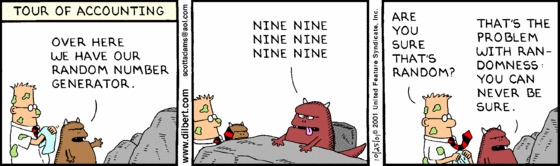
\includegraphics[width=17cm]{images/ninenine.png}
  \caption{Dilbert, «We guarantee that each number is random individually,
  but we don't guarantee that more than one of them is random»,
  \url{http://en.wikipedia.org/wiki/RANDU}}
\end{figure*}

\begin{sol}
  Да. Например, такая.
  До общения с Машей подкидывать монетку до выпадения первого орла
  и запомнить число потребовавшихся подбрасываний. Пусть это будет число $X$.
  Открыть равновероятно левую или правую Машину руку. Если открытое число больше $X$,
  то сказать, что оно большее, иначе сказать, что меньшее.
\end{sol}


\end{problem}


\begin{problem}
Больший кусок окружности

Аня хватается за верёвку в форме окружности в произвольной точке.
Боря берёт мачете и с завязанными глазами разрубает
верёвку в двух случайных независимых местах. Аня забирает себе тот кусок,
за который держится. Боря забирает оставшийся кусок. Вся верёвка имеет единичную длину.
\begin{enumerate}
\item Чему равен ожидаемый длина куска верёвки, доставшегося Ане?
\item Вероятность того, что у Ани верёвка длиннее?
\end{enumerate}

\begin{sol}
  \begin{enumerate}
  \item Мысленно отметим на окружности три точки: места ударов Бориса и точку,
  где схватилась Анна. Можно считать, что эти три точки равномерно
  и независимо распределены по окружности.
  Следовательно, среднее расстояние между соседними точками равно $1/3$.
  Аня берёт два кусочка, слева и справа от своей точки.
  Значит ей в среднем достаётся $2/3$ окружности.
  \item  Объявим точку, где схватилась Аня нулём.
  Координаты двух ударов изобразим на плоскости. Закрашиваем подходящий участок.
  Аня выигрывает на полосе вдоль биссектрисы за исключением двух треугольников.
  Вероятность того, что Анин кусок длиннее равна $3/4$.
  \end{enumerate}
\end{sol}


\end{problem}


\begin{problem}
Судьба Дон-Жуана.

У Дон-Жуана $n$  знакомых девушек, и их всех зовут по-разному. Он пишет
им $n$  писем, но по рассеянности раскладывает их в конверты
наугад. Случайная величина $X$ обозначает количество девушек, получивших письма,
адресованные лично им.

\begin{enumerate}
\item Найдите $\E(X)$, $\Var(X)$
\item Какова при большом $n$ вероятность того, что хотя бы одна девушка получит письмо,
адресованное ей?
\end{enumerate}

\begin{sol}
Раскладываем $X$ в сумму $X=Z_1 + Z_2 + \ldots + Z_n$. Получаем, $\E(X)=1$, $\Var(X)=1$.
\end{sol}

\end{problem}


\begin{problem}
Ефросинья подкидывают правильную монетку неограниченное количество раз.

\begin{enumerate}
\item Сколько в среднем нужно сделать бросков до появления последовательности ОРОР?
До появления последовательности РОРР?
\item Какова вероятность того, что ОРОР появится раньше РОРР?
\item Какова вероятность того, что ООО появится позже РРОО?
\item Каковы вероятности того, что ООР появится раньше ОРР? ОРР раньше РРО?
РРО раньше РОО? РОО раньше ООР?
\end{enumerate}

\begin{sol}
\begin{enumerate}
\item Воспользуемся интересным методом, который описан в статье \cite{li1980martingale}.

Метод заключается в том, что игроки учавствуют в честной лотерее.
Если поставил $1$\$: выиграл – получаешь $2$, включая поставленный $1$;
проиграл – у тебя $0$.

Допустим у нас есть последовательность ОРРРОРОР. Выигрышная последовательность ОРОР.
Все ставят на то, что в следующий ход выиграет эта комбинация следующим образом.
Ставится $1$\$ на то, что выпадет О. Если выпадает О,
то игрок обязан поставить полученные $2$ доллара на Р. Если опять выиграл,
то обязан поставить все $4$ выигранных доллара на Р и так далее.
Если проиграл, то выбывает игрок теряет деньги и выбывает из игры.

Кроме того, игроки вступают в игру так: в первый раз ставит 1 игрок,
во второй раз игроки 1 и 2 (если 1 не проиграл до этого),
в третий раз учвствуют игроки 1, 2, 3
(опять же, если один или оба не выбыли в результате прошлого кона).

В конце концов считается чистый выигрыш и ожидемое колличество бросков.

В нашем случае что-то выиграют 5 и 7 игроки (у 5 выигрыш равен $16$, у 7 – $4$).

Чистый выигрыш = $20 - N$, где $N$ - колличество ходов до ОРОР.
Организованная лотерея имеет нулевое математическое ожидание выигрыша на каждом ходу,
значит мат ожидание финального благосостояния игрока равно стартовому благосостоянию.
Тогда $\E(N) = 20$.

Итого, ожидаемое колличество ходов: до $\text{ОРОР} = 16 + 4 = 20$,
до $\text{РОРР} = 16 + 2 =18$.

Есть и ещё один метод решения, изложенный в
«DNA, Words And Models» by Robin, Rodolphe, and Schbath. Авторы объясняют,
почему математическое ожидание есть сумма обратных вероятностей каждого префикса в слове,
который также является суффиксом этого же слова.
В случае ОРОР такие суффиксы-префиксы — это ОРОР и ОР, в случае РОРР это РОРР и Р.
Удивительно, но результат окажется таким же, как при предыдущем методе решения.

А вообще, это все можно вывести самостоятельно, вот пример,
если нужно найти количество бросков до ОРО:
\[
\begin{aligned}
\E(0) &= \frac{1}{2} (\E(\text{О}) + 1) + \frac{1}{2} (\E(0) + 1)\\
\E(\text{О}) &= \frac{1}{2} (\E(\text{О}) + 1) + \frac{1}{2} (\E(\text{ОР}) + 1)\\
\E(\text{ОР}) &= \frac{1}{2} (\E(\text{ОРО}) + 1) + \frac{1}{2} (\E(0) + 1)\\
\E(\text{ОРО}) &= 0
\end{aligned}
\]

По аналогии можно найти и количество бросков до ОРОР, и до РОРР
\item Пусть у меня есть какие-то состояние $p_{0,0}$ – это верятность того,
что ОРОР появится раньше РОРР, но еще не выпал ни орел, ни решка.

Тогда с вероятностью $0.5$ я окажусь в состоянии $p_{0,1}$ (выпала решка) и с $0.5$
в состоянии $p_{1,0}$ (выпал орел).

Получаем: $p_{0,0}=0.5p_{0,1}+0.5p_{1,0}$.

Таким образом, в конце концов можно составить систему
\[
\begin{cases}
2p_{0,0}=p_{0,1}+p_{1,0}\\
2p_{0,1}=p_{0,1}+p_{1,2}\\
2p_{1,0}=p_{2,1}+p_{1,0}\\
2p_{1,2}=p_{2,3}+p_{1,0}\\
2p_{2,1}=p_{0,1}+p_{3,2}\\
2p_{2,3}=p_{0,4}+p_{3,2}=p_{3,2}\\
2p_{3,2}=p_{4,3}+p_{0,0}=1+p_{1,0}\;,
\end{cases}
\]
где $p_{0,4} = 0$ и $p_{4,3} = 1$

Можно переписать систему как
\[
\begin{cases}
2p_{0,0}=p_{1,2}+p_{2,1}\\
2p_{1,2}=p_{2,3}+p_{2,1}\\
2p_{2,1}=p_{1,2}+2p_{2,3}\\
4p_{2,3}=1+p_{2,1}\;,
\end{cases}
\]
Решив ее, получаем ответ $p_{0,0} = 9/14$
\item Воспользуемся методом из Section 8.4 («Flipping Coins») из Concrete Mathematics.
Найдему сумму всех возможных кобинаций,

где побеждает РРОО: $S_{1} = \text{РРОО} +\text{ОРРОО}+\text{РРРОО}+\text{ОРРРОО}+\text{РОРРОО}+\ldots $

где побеждает ООО: $S_{2} = \text{ООО}+ \text{РООО}+\text{ОООО}+\text{ОРООО}+\ldots $

где никто не побеждает: $N= 1 + \text{О}+\text{Р}+\text{ОР}+\text{ОО}+\text{РО}+\ldots $

Тогда, если мы заменим О и Р на вероятности их появления ($0.5$ и $0.5$),
то получим вероятность победы первой комбинации,
вероятность выигрыша второй комбинации и матемачиское ожидание окончания игры.

Составим три уравнения:
\[
\begin{cases}
N \text{ООО} = S_{2} +S_{2} \text{О} + S_{2}\text{ОО} + S_{1}\text{О} + S_{1} \text{ОО}\\
N \text{РРОО} = S_{1} \\
S_{1} + S_{2} = 1\\
\end{cases}
\]
То есть мы к $N$ добавляем искомые комбинации и смотрим, как это всё расскладывается.

Ответ: $\P = 0.58333333$

\item ООР раньше чем ОРР? Не будем долго думать и воспользуемся уже известным способом
\[
\begin{cases}
N \text{ООР} = S_{1}\\
N \text{ОРР} = S_{2} +S_{1} \P\\
S_{1} + S_{2} = 1\\
\end{cases}
\]

$\P = 0.66666667$

ОРР раньше РРО?
\[
\begin{cases}
N \text{ОРР} = S_{1}  + S_{2}\text{РР}\\
N \text{РРО} = S_{2}+ S_{1} \text{РО}+S_{1} \text{О}\\
S_{1} + S_{2} = 1\\
\end{cases}
\]

$\P = 0.75$

РРО ранше РОО?
\[
\begin{cases}
N \text{РРО} = S_{1} \\
N \text{РОО} = S_{2}+ S_{1} \text{О}\\
S_{1} + S_{2} = 1\\
\end{cases}
\]

$\P = 0.66666667$

РОО раньше ООР?
\[
\begin{cases}
N \text{РОО} = S_{1} + S_{2} \text{ОО}\\
N \text{ООР} = S_{2} +S_{1} \text{ОР} +S_{1} \text{Р}\\
S_{1} + S_{2} = 1\\
\end{cases}
\]

$\P = 0.75$
\end{enumerate}
\end{sol}

\end{problem}


\begin{problem}
Илье Муромцу предстоит дорога к камню. От камня начинаются ещё три дороги.
Каждая из тех дорог снова оканчивается камнем.
И от каждого камня начинаются ещё три дороги.
 И каждые те три дороги оканчиваются камнем\ldots И так далее до бесконечности.
 На каждой дороге живёт трёхголовый Змей Горыныч.
 Каждый Змей Горыныч бодрствует независимо от других с вероятностью
 (хм, Вы не поверите!) одна третья.
 У Василисы Премудрой существует Чудо-Карта, на которой видно,
 какие Змеи Горынычи бодрствуют, а какие — нет.

 Какова вероятность того, что Василиса Премудрая сможет найти на карте
 бесконечный жизненный путь Ильи Муромца,
 проходящий исключительно мимо спящих Змеев Горынычей?


\begin{sol}
Пусть дорога к первому камню — дорога $a$; эта дорога соединяет
начальное положение ИМ и первый камень. От первого камня идут три дороги:
$c, \; d,\text{ и }e$. Ищем вероятность $p_a$ —
вероятность пройти бесконечный жизненный путь, начиная с дороги $a$.

Заметим, что существование бесконечного жизненного пути,
начинающегося дорогой $a$ — пересечение двух независимых событий:
на дороге $a$ ЗГ спит и существует бесконечный жизненный путь,
начинающийся хотя бы одной из дорог $c, \; d, \; e$.
~\\

$\P \text{\{на дороге } a \text{ ЗГ спит\}} = \frac{2}{3}$
~\\

Пусть $p_c,\; p_d$ и $p_e$ — вероятности того, что существуют бесконечный жизненный путь,
начинающийся дорогой $c, \; d, \; e$ соответственно. Теперь заметим,
что $p_a=p_c= p_d=p_e$, т. к. рассматривается возможность идти бесконечно.
Обозначим $p = p_a$; получаем уравнение:
\[
p = \frac{2}{3}\left(1 - (1-p)^3\right)
\]

У него три решения, одно из которых больше $1$. Два других:
\begin{center}
\begin{minipage}{52mm}
$p_1=0$
\end{minipage}
\hspace{0mm}
\begin{minipage}{22mm}
$p_2=\frac{3 - \sqrt{3}}{2}$
\end{minipage}
\end{center}

Определим, каким из этих двух значений может быть равна искомая вероятность $p_a$
\footnote{Интуитивно понятно, что $p_1=0$ едва ли может быть решением задачи,
поскольку такое решение уравнения не зависит от вероятности встретить бодрствующего ЗГ.
Если бы вероятность встретить его была бы $0$, то есть
если бы бесконечный жизненный путь точно бы существовал,
у уравнения всё равно был бы корень $p=0$. Однако докажем строго,
что решением будет положительная величина.}.

Пусть ЗГ появляется на дороге с вероятностью $\alpha$. Уравнение примет вид:
\[
p = \alpha\left(1 - (1-p)^3\right)
\]
Одним из решений уравнения всегда будет $p=0$,
другим, всегда лежащим в интервале $(0;1)$,
— $p=\frac{3\alpha - \sqrt{4\alpha-3\alpha^2}}{2\alpha},(\alpha\neq0)$.

Такое решение монотонно возрастает, является положительным
на промежутке $\alpha \in \left(\frac{1}{3};\; 1\right]$. При $\alpha=1 \; p = 1$.

Теперь вернёмся к функции $p(\alpha)$. Поскольку она означает зависимость
вероятности существования бесконечного пути от вероятности того, что ЗГ спит,
ясно, что эта функция монотонна, непрерывна и неотрицательна,
а так же должна принимать значение $0$ при $\alpha=0$ и значение $1$ при $\alpha=1$.

Следовательно, функция $p(\alpha)$ будет иметь следующий вид:

\[
p(\alpha)=\begin{cases}
0,\alpha \in \left[0; \frac{1}{3}\right]\\
\frac{3\alpha - \sqrt{4\alpha-3\alpha^2}}{2\alpha}, \; \alpha \in \left(\frac13;1\right]
\end{cases}
\]

Получаем, что при данном в этой задаче $\alpha=\frac23$, искомая вероятность
составит $\frac{3 - \sqrt{3}}{2}$.
\end{sol}
\end{problem}

\begin{problem}
У тёти Маши — двое детей разных возрастов. Вероятности рождения мальчика и девочки равны.

\begin{enumerate}
\item Какова вероятность того, что у тёти Маши оба ребёнка — мальчики, если известно,
что у неё хотя бы один ребёнок — мальчик?
\item Какова вероятность того, что у тёти Маши оба ребёнка — мальчики, если известно,
что у неё хотя бы один ребёнок — мальчик водолей по гороскопу?
\end{enumerate}

\begin{sol}
\begin{enumerate}
\item Для краткости: $M$ — мальчик, $F$ — девочка.

Возможные исходы: MM, FF, MF, FM.

Нужно найти условную вероятность:
\[
\P(\text{MM | хотя бы один M}) =
\frac{\P(\text{MM} \cap \text{хотя бы один M})}{\P(\text{хотя бы один M})} =
\frac {1/4}{3/4} = \frac{1}{3}
\]

\item Нужно найти условную вероятность:
\[
\P(\text{M | хотя бы один M водолей}) =
\frac{\P(\text{MM} \cap \text{хотя бы один M водолей)}}
{\P(\text{хотя бы один M водолей})}
\]
Поскольку вероятность того, что конкретный ребёнок — мальчик-водолей равна $1/24$,
то в знаменателе будет:
\[
\P( \text{хотя бы один M водолей}) = 1 - \left(\frac{23}{24}\right)^2
\]
Чтобы посчитать числитель, заметим, что событие «оба мальчика,
хотя бы один мальчик водолей» эквивалентно событию «оба мальчика,
хотя бы один ребёнок водолей», тогда,
воспользовавшись независимостью пола от знака зодиака, получим:
\begin{equation*}
\begin{split}
\P(\text{ММ, хотя бы один M водолей}) &=  \P(\text{ММ, хотя бы один ребёнок водолей}) \\
 &= \frac{1}{4} \P(\text{хотя бы один ребёнок водолей})\\
  &= \frac{1}{4}(1-\P(\text{оба ребёнка не водолеи})) \\
&=\frac{1}{4}\left(1 - \left(\frac{11}{12}\right)^2\right)
\end{split}
\end{equation*}
В итоге получаем:
\[
\P(\text{MM | хотя бы один M водолей}) =
\frac{\frac{1}{4}\left(1 - \left(\frac{11}{12}\right)^2\right)}
{1 - \left(\frac{23}{24}\right)^2} = \frac{23}{47} \approx 0.489
\]

%\todo[inline]{проверить! интуитивно около 1/2 должно быть}

\end{enumerate}
\end{sol}

\end{problem}


%%%%%%%%%%%%%%%%%%%%%%%%%%%%%%%%%%%%%%%%%%%%%%%%%%%%%%%%%%%%%%%
%%% убираем длинные абзацы :)
%%%%%%%%%%%%%%%%%%%%%%%%%%%%%%%%%%%%%%%%%%%%%%%%%%%%%%%%%%%%%%%

\begin{problem}
Buffon's needle problem

Плоскость разлинована параллельными линиями через каждый сантиметр.
Случайным образом на эту плоскость бросается иголка длины $a<1$.

\begin{enumerate}
\item Какова вероятность того, что иголка пересечёт какую-нибудь линию?
\item Предложите вероятностный способ оценки числа $\pi$
\end{enumerate}

\begin{sol}
Поскольку $a<1$ количество пересечений равно либо 0, либо 1, следовательно,
вероятность пересечения равна математическому ожиданию числа пересечений.
Обозначим $X$ — количество пересечений. Если иголку удлиннить в $n$ раз,
то $\E(X)$ изменится в $n$ раз, так как фактически мы имеем $n$ иголок равной длинны.
Если иголку согнуть в ломаную, то $\E(X)$ не меняется,
так как снова иголка разрезается на отдельные иголки. Отсюда получаем,
что $\E(X)$ зависит только от длины иголки, но не от формы.
Сгибаем иголку в окружность. Если длина равна $\pi$, то пересечений будет два.
Значит при длине $a$ ожидаемое количество пересечений равно $2a/\pi$.
\end{sol}


\end{problem}


\begin{problem}
Мартышка и Шекспир

Мартышка наугад нажимает клавиши на печатающей машинке.


\begin{enumerate}
\item Какова вероятность того, что она рано или поздно напечатает
полное собрание сочинений Шекспира? Льва Толстого?
\item Обозначим количество нажатий до появления слова «АБРАКАДАБРА» за $X$.
Найдите $\E(X)$ и $\Var(X)$.
\end{enumerate}


\begin{marginfigure}
  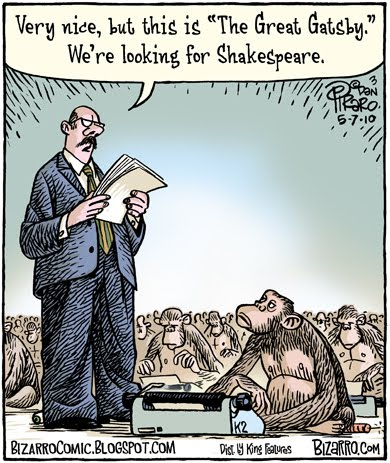
\includegraphics[width=5cm]{images/gatsby}
  \caption{Задача о «бесконечных обезьянах», infinte-monkey problem. }
\end{marginfigure}

\begin{sol}
\begin{enumerate}
\item Для начала стоит обратить внимание на кажущуюся незаметной,
но довольно важную фразу: «рано или поздно».
Вероятность искомого события стремится к единице при условии стремления
времени к бесконечности. Таким образом, каким бы невероятным не было утверждение о том,
что обычная мартышка, наугад нажимающая клавиши на печающей машинке,
рано или поздно напечатает собрание сочинений Шекспира или Льва Толстого,
оно тем не менее является достоверным.

Докажем данное утверждение в более явном виде. Как мы знаем из курса тервера,
два события независимы, если вероятность пересечения событий равна произведению
вероятностей этих событий.

Теперь предположим, что пишущая машинка имеет $50$ клавиш. Допустим,
перед мартышкой стоит задача напечатать слово «обезьяна». Вероятность того,
что первым напечатанным символом станет буква «о», равна $1/50$, ровно как и
вероятность того, что следующим символом станет буква «б» и так далее,
поскольку эти события независимы. Таким образом, вероятность того, что
мартышка напечатает заданное слово, равна $\frac{1}{50^6}$.

С другой стороны, шанс не напечатать слово «обезьяна» в каждом блоке по $8$ букв
равен $1 - \frac{1}{50^6}$. Поскольку каждый блок печатаетcя независимо,
шанс не напечатать данное слово в любом из первых $n$ блоков по $8$ букв
равен $\left(1 - \frac{1}{50^6}\right)^n$. Причём в данном случае найденная
формула может быть интерпретирована как вероятность того,
что ни одна из $n$ обезьян не напечатает слово «обезьяна» правильно с первой попытки.
Более того, из этой формулы видно, что чем больше $n$, тем меньше данная вероятность.

Подобная формула применяется для любой другой строки символов конечной длины.
При этом если заменить слово «обезьяна» на текст «Гамлета»,
показатель степени увеличится с $8$ до числа символов в этом тексте,
но суть от этого не изменится. Таким образом, если устремить $n$ к бесконечности,
выражение $\left(1 - \frac{1}{50^6}\right)^n$ будет стремиться к нулю.
Иными словами, при бесконечном количестве обезьян вероятность
не напечатать текст любой сложности будет близка к нулю.
Однако условие наличия бесконечного количества обезьян равносильно
условию наличия одной обезьяны, печатающей при неограниченном количестве времени.

В результате получаем, что вероятность того, что одна обезьяна рано или поздно
не напечатает полное собрание сочинений Шекспира стремится к нулю,
значит вероятность того, что она его напечает, стремится к единице.

\item Обозначим количество нажатий до появления слова «абракадабра» за $X$.
Найдём $\E(X)$.

%\todo[inline]{Мы в России! 33!}

Для упрощения ситуации предположим, что на печатной машинке есть всего $33$ кнопок,
соответствующих $33$ буквам русского алфавита.

Первоначально можно рассуждать следующим образом:
вероятность правильно напечатать нужную букву из $33$ возможных равна $\frac{1}{33}$,
а вероятность правильно напечатать нужные $11$ букв подряд соответственно
равна $\frac{1}{33^{11}}$. Таким образом, если набор $11$ букв это одно испытание,
то математическое ожидание количества испытаний
равно $\frac{1}{\frac{1}{33^{11}}} = 33^{11}$.

Однако данный ответ является не совсем точным.

Для нахождения точного математического ожидания $X$ смоделируем следующую ситуацию.
Допустим, что мы открываем справедливое казино, суть которого заключается в том,
что перед каждым нажатием обезьяной клавиши к нам приходит новый игрок и
ставит 1 д.е. на определенную букву. Так, вначале игрок поставит на букву «а».
Если он не угадывает, то уходит домой. Если же он угадывает,
то ставит все выигранные деньги на то, что следующая буква будет «б».
В случае очередного выигрыша, он ставит на то, что следующая буква будет «р»
и так далее.

Данная игра продолжается до тех пор, пока не появится слово «абракадабра»
(за искомое количество нажатий $X$). После появления данного слова мы закрываем казино.

Поскольку казино справедливое, математическое ожидание выигрыша равно нулю.
Таким образом, если игрок ставит 1 д.е., он должен получить 33 д.е,
поскольку вероятность правильно угадать букву как раз равна $\frac{1}{33}$.
В итоге — ожидаемое изменение в благосостоянии игрока
равно $\frac{32}{33}\cdot(-1) + \frac{1}{33}\cdot(+32) = 0$.

Как уже было сказано, игра длится $X$ нажатий. Сколько заработает наше казино?
Напомним, что перед каждым нажатием клавишы новый игрок приходит и ставит 1 д.е.
и, если он выигрывает, он будет ставить только все деньги, которые заработал.
Поэтому наша выручка будет в точности равна $X$ д.е.

Сколько наше казино заплатит победителям? Заметим,
что победителями в последнем раунде становятся те, кто ставит на «а».
Существует один игрок, который пришел в казино перед последней буквой
и выиграл $33$ д.е. на своей ставке. Также был игрок,
который пришел тремя нажатиями ранее, он сделал четыре успешные ставки («абра»)
и выиграл соответственно $33^4$. Наконец, существует наиболее успешный игрок,
который прошел через все слово «абракадабра» и выиграл $33^{11}$.
Таким образом, наше казино должно отдать $33^{11}+33^4+33$ д.е. в итоге.

Наконец, сделаем следующее уточнение: наше казино является справедливым,
даже когда мы его закрываем. Поэтому расходы казино должны быть равны доходам казино.
Наш доход равен $X$ д.е, в то время как ожидаемые расходы равны $33^{11}+33^4+33$,
поэтому $\E (X - (33^{11}+33^4+33)) = 0$. Откуда $\E(X) = 33^{11}+33^4+33$.

Что касается $\Var(X)$, данную величину можно найти аналогичным способом,
записав другое уравнение вида $\E(X^2 - T)=0$, где $T$ – совокупное
благосостояние всех игроков (напомним, что наше казино справедливое,
поэтому правая часть данного уравнения приравнивается к $0$).
Отсюда найдем $\E(X^2)$, а величина $(\E(X))^2$
соответственно равна $(33^{11}+33^4+33)^2$ из предыдущего пункта.
\end{enumerate}
\end{sol}

\end{problem}


\begin{problem}
Парадокс инспектора

Автобусы приходят на остановку согласно пуассоновскому потоку в среднем один раз в час.
Вася приходит на остановку в случайный момент времени и садится
на первый пришедший автобус.

\begin{enumerate}
\item Сколько Васе в среднем предстоит ждать автобуса?
\item Сколько в среднем прошло времени от последнего пришедшего автобуса
до Васиного появления?
\item Чему равна средняя продолжительность интервала между автобусом,
на который сядет Вася, и предыдущим?
\item Чему равна средняя продолжительность интервала между автобусом,
на который сядет Вася, и следующим?
\item Маша не любит набитые битком автобусы и никогда не торопится, поэтому,
придя на остановку, всегда пропускает один автобус и садится на следующий.
Она считает, что на него в среднем сядет меньше людей. Права ли она?
\end{enumerate}


\begin{sol}
Да, Маша права, на «следующий» в среднем садится меньше пассажиров.
\end{sol}

\end{problem}


\begin{problem}
Спящая красавица

Спящая красавица согласилась принять участие в научном эксперименте.
В воскресенье её специально уколют веретеном. Как только она заснёт,
будет подброшена правильная монетка.


Если монетка выпадет орлом, то спящую красавицу разбудят в понедельник
и спросят о том, как выпала монетка.


Если монетка выпадет решкой, то спящую царевну разбудят в понедельник,
спросят о монетке, снова уколют веретеном, разбудят во вторник
и снова спросят о монетке. Укол веретена вызывает легкую амнезию,
и красавица не сможет определить, просыпается ли она в первый раз или во второй.

Красавица только-только проснулась. Вспомнила правила эксперимента,
и услышала вопрос исследователя: «Ваше Высочество, так как же выпала монетка?»
\begin{enumerate}
\item Как следует отвечать красавице, если за каждый верный ответ ей
дарят молодильное яблоко?
\item Как следует отвечать красавице, если за неверный ответ её тут
же превращают в тыкву?
\item Отвечая на вопрос исследователя Спящая Красавица задумалась,
а какова вероятность того, что сегодня понедельник. Как ты думаешь?
\end{enumerate}



\begin{sol}
«Сегодня понедельник» — это \textbf{не} событие. Вероятность не
определена. Это функция от времени.

Вероятность того, что монетка выпала орлом, равна $0{,}5$. Поэтому ей
всё равно, как отвечать, если наказанием является превращение в
тыкву, и нужно отвечать: «Решка!» — если наградой является
молодильное яблоко. Предположим, что красавица максимизирует
ожидаемое количество молодильных яблок.
\end{sol}

\end{problem}


\begin{problem}
Monty-Hall

Есть три закрытых двери. За двумя из них — по козе, за третьей автомобиль.
Вы выбираете одну из дверей. Допустим, Вы выбрали дверь А.
Ведущий шоу, чтобы поддержать интригу, не открывает сразу выбранную Вами дверь.
Сначала он открывает одну из дверей не выбранных Вами,
причем ради интриги ведущий не открывает сразу и дверь с автомобилем.
Допустим, ведущий открыл дверь B. И в этот момент он предлагает Вам
изменить ваш выбор двери.

Имеет ли смысл изменить свой выбор?

\begin{figure*}
  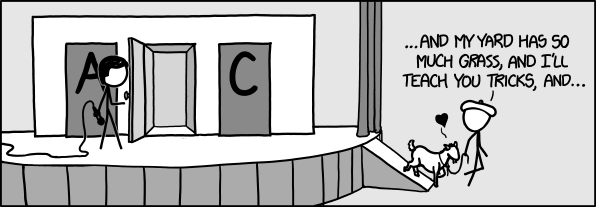
\includegraphics[width=17cm]{images/monty_hall}
  \caption{A few minutes later, the goat from behind door C drives away in the car.
  \url{http://xkcd.com/1282/}}
\end{figure*}

\begin{sol}
Перед игроком три двери А, Б, В. Пусть он выбрал А. Тогда,
если он поменяет свой выбор после хода судьи, то проигрыш наступит только,
если в самом начале игрок выбрал дверь, за которой находится автомобиль,
т.к. впоследствии он изменит своё решение в пользу двери с козой,
во всех остальных случаях он выиграет, то есть,
если с самого начала ошибся с выбором двери.
А вероятность с самого начала выбрать дверь с козой $2/3$.
Если же он не поменяет свой выбор, то вероятность ошибиться
в первый (и единственный) ход равна $2/3$, а угадать автомобиль, соответственно, $1/3$.
В итоге вероятность выиграть автомобиль равна $2/3$, если поменять выбор,
и $1/3$, если не менять выбор.

Ответ: игроку нужно изменить свой выбор.
\end{sol}

\end{problem}


\begin{problem}
Monty-Hall версия

Трое студентов, Аня, Боря и Василиса, сдавали комиссию по теории вероятностей
и ещё не знают своих оценок. Им объявили, что зачёт получили двое из трёх.
В перерыве перед объявлением оценок Боря подходит к председателю комиссии:

— Иван Иванович, раз зачёт получили двое из трёх,
значит хотя бы у одной из девушек есть зачёт. Вы мне можете назвать имя
одной из девушек, получившей зачет?

— Василиса получила.

Какова условная вероятность того, что Боря получил зачёт,
если принимать во внимание информацию от Ивана Ивановича?

\begin{sol}
По-прежнему $2/3$.
\end{sol}

\end{problem}


\begin{problem}
Задача о Разборчивой Невесте, Secretary problem

К Разборчивой невесте выстроилась длинная-длинная вереница из потенциальных женихов.
\marginnote{Докторская диссертация член-корреспондента РАН Бориса Березовского
«Разработка теоретических основ алгоритмизации принятия предпроектных решений и их применения»
является обобщением задачи о разборчивой невесте, \url{http://en.wikipedia.org/wiki/Secretary_problem}}
Разборчивая невеста хочет выбрать самого богатого из них и только его!
Потенциальные женихи заходят к Разборчивой невесте по одному в случайном порядке.
Невеста неплохо разбирается в богатстве и легко может ранжировать всех, с кем она общалась,
по величине богатства. Когда к Разборчивой невесте приходит очередной претендент,
она должна сразу принять решение: выбрать данного кандидата или перейти к следующему.
Вернуться к предыдущим кандидатам невозможно — они обижаются и уезжают.

\begin{enumerate}
\item Как выглядит оптимальная стратегия Разборчивой невесты?
Чему равна вероятность выбора самого богатого жениха Разборчивой невестой?
\item Подруга-дурнушка Разборчивой невесты хочет
выбрать второго по богатству жениха и только его!
\marginnote{Всё равно самый богатый достанется Разборчивой невесте!}
Как выглядит её оптимальная стратегия? Чему равна вероятность выбора
второго по богатству жениха Подругой-дурнушкой?
\end{enumerate}

\begin{sol}

Разберёмся сначала с Разборчивой невестой!

На русском хорошо написана короткая книжка \cite{zade2003nevesta}.
Про подружку, согласную на второго красавца, изложено в \cite{vanderbei2011postdoc}.

Входит претендент номер $k$. Назовём претендента приемлемым, если он лучше предыдущих,
и неприемлемым иначе. Если вошёл неприемлемый претендент, ему оптимально отказать.
Найдем вероятности выигрыша:

\begin{enumerate}
  \item Вероятность выигрыша, если кандидат номер $k$ — наилучший и мы его примем, $f_k$.
  \item Вероятность выигрыша, если отвергли кандидата номер $k$, $v_k$.
\end{enumerate}

Замечаем, что если мы отказали, то вероятность выигрыша не зависит от того,
кому мы отказали, приемлему кандидату или неприемлемому.


Выбор приемлемого кандидата приводит к победе, если он — наилучший из всех, или,
другими словами, если наилучший из всех $n$ претендентов попался на первые $k$ мест.
Следовательно, эта вероятность равна $f_k = k/n$.

Осталась вероятность $v_k$. Если мы отказали кандидату номер $k$, то следующий
окажется приемлемым с вероятностью $1/(k+1)$. Это ровно вероятность того, что
из $k+1$ кандидата наилучший окажется последним. Поэтому
\[
v_k = \frac{1}{k+1} \max \{v_{k+1}, f_{k+1} \} + \frac{k}{k+1} v_{k+1}
\]

Решая с конца находим, что вплоть до момента остановки $v_k = ....$.


Альтернативное решение можно построить с помощью стратегии «Складывай шансы до единицы!».
Идея принадлежит \cite{bruss2000sum}, хотя есть и гораздо более простое доказательство.

Шансы (odds) — это отношение вероятности успеха к вероятности неудачи.

Замечаем, что вероятность того, что $k$-ый кандидат лучше предыдущих равна $1/k$.
Следовательно, шансы равны $(1/k)/(1-1/k)=1/(k-1)$. Согласно стратегии «Складывай шансы до единицы!»
оптимальный порог — это наибольшее $m$, такое, что выполнено условие

\[
\frac{1}{n-1} + \frac{1}{n-2} + \ldots + \frac{1}{m-1} \geq 1
\]


Теперь разбираемся с подружкой Разборчивой невесты. Представляем ситуацию, что к нам
входит очередной кандидат $k$. Рассмотрим вероятности выигрыша в каждом
из случаев:

\begin{enumerate}
  \item Вероятность выигрыша, если кандидат номер $k$ — второй лучший и мы его примем, $g_k$.
  \item Вероятность выигрыша, если кандидат номер $k$ — наилучший и мы его примем, $f_k$.
  \item Вероятность выигрыша, если отвергли кандидата номер $k$, $v_k$.
\end{enumerate}

Замечаем, что $v_k$ не зависит от того, кого мы отвергли только что, так как ранги
будущих претендентов не зависят от прошлого.

По смыслу $g_k$ — это вероятность того, что второй лучший из $k$ человек является вторым
лучшим из $n$ человек. Такое может произойти, если второй лучший из $n$ человек попал
на одно из первых $k$ мест, а самый лучший попал на $k-1$ оставшееся место из $n-1$.

Безо всякой индукции получаем сразу, что $g_k = \frac{k}{n}\frac{k-1}{n-1}$.

Аналогично находим вероятность $f_k$. По определению, это вероятность того, что наилучший
из $k$ человек является вторым лучшим из $n$. Такое может произойти, если второй лучший из
$n$ человек попал на одно из первых $k$ мест, а самый лучший попал на одно из $n-k$ оставшихся
мест.

Поэтому $f_k = \frac{k}{n}\frac{n-k}{n-1}$.

Рассмотрим $k<n$. Если мы откажем кандидату $k$, то:
\begin{enumerate}
  \item С вероятностью $1/(k+1)$ новый кандидат будет наилучшим из $k+1$;
  \item С вероятностью $1/(k+1)$ новый кандидадт будет вторым лучшим из $k+1$;
  \item С вероятностью $(k-1)/(k+1)$ новый кандидат будет заведомо проигрышным.
\end{enumerate}

Поэтому:
\[
v_k = \frac{k-1}{k+1}v_k + \frac{1}{k+1}\max\{v_{k+1}, f_{k+1}\}  +
\frac{1}{k+1}\max\{v_{k+1}, g_{k+1}\}
\]

Решая с конца находим, что оптимально отбросить
первых $k_0 = \lfloor n/2 \rfloor$ кандидатов.
А далее можно согласиться на первого кандидата,
являющегося вторым наилучшим среди уже осмотренных.

\todo[inline]{...}


\end{sol}

\end{problem}


\begin{problem}
Собрались как-то вместе много-много ковбоев, а именно в количестве $n$ человек.
Каждый из них выбрал себе из остальных своего самого главного врага случайным образом.
Далее ковбои по очереди стреляют, каждый в своего главного врага.
Естественно, если жив сам, и если жив самый главный враг.
Ковбои стреляют без промаха.
\begin{enumerate}
\item Какая доля ковбоев в среднем останется в живых?
\item Какая доля ковбоев в среднем останется в живых,
если треть ковбоев забыла дома свой кольт?
\end{enumerate}


\begin{sol}
\begin{enumerate}
\item Имеется $n$ ковбоев. Каждый из них может быть либо жив, либо мертв.
Пусть $X_i$ – случайная величина, которая может быть равна $1$ или $0$ в случае,
если ковбой жив и убит соответственно. Тогда матожидание от выживших –
это сумма матожиданий от каждой случайной величины $X_i$.
Но раз они независимые и биномиально распределенные,
тогда матожидания всех равны между собой.
Поэтому итоговое матожидание равно $\E(X) = n\E(X_{i})$.
Поэтому необходимо найти матожидание от одной случайной величины.
Но раз мы знаем, что она распределена биномиально, тогда ее матожидание
будет равно $0\cdot\P(\text{случайно выбранный ковбой умрёт})+
1\cdot\P(\text{случайно выбранный ковбой выживет})$.

$\P(\text{случайно выбранный ковбой выживет}) =1/2$.  Тогда итоговое матожидание=$n/2$.

Можно ещё сделать через матиндукцию. Для случая $n=2$ матожидание легко считается,
и оно равно $1$. Предположим, что у нас доказано для $n-1$,
что матожидание равно $\frac{n-1}{2}$. Далее скажем, что сейчас у нас есть $n$ ковбоев.
Тогда можем сказать, что всегда найдется тот, кто стреляет последним.
Это значит, что из остальных никто в него не целился, либо тот,
кто целился, был убит. Более того, еще нам неважно, куда он целился.
Тогда можно сказать, что все остальные $n-1$ целились только друг в друга.
Здесь срабатывает наша предпосылка о матожидании для $n-1$ человек.
Среди этих человек матожидание $\frac{n-1}{2}$. Также из предположения индукции
мы знаем, что вероятность того, что ковбой выживает $1/2$,
а значит, мы (точнее, этот ковбой, который стреляет последний) целимся
в живого человека с вероятностью $1/2$. Тогда мы можем либо убить его,
либо нет с равной вероятностью. Учитываем в нашем матожидании оба случая.
Тогда, если мы его не убиваем, тогда остаётся $((n-1)/2)+1$
человек с вероятностью $1/2$. Если же убиваем,
тогда останется $\left(\frac{n-1}{2}\right) -1+1$. Здесь мы вычли того,
кого убили, и добавили нас.

Ответ: матожидание = $\left(\frac{n-1}{2}+1\right)\cdot\left(\frac{1}{2}\right)+
\left(\frac{n-1}{2}\right)\cdot\left(\frac{1}{2}\right)=
\left(\frac{n+1}{4}\right)+\left(\frac{n-1}{4}\right)=\frac{n}{2}$

\item Если же у нас ровно $1/3$ ковбоев забыла свой кольт, тогда вероятность того,
что случайно выбранный ковбой останется в живых повышается.
То есть новая вероятность будет равна: $\frac{1}{2-X}$, где $X$ – доля тех ковбоев,
кто не взял с собой свой кольт. Значит, наша вероятность будет равна $\frac{3}{5}$.
Также известно, что наши случайные величины соответствуют $0$, если ковбой убит,
и $1$, если ковбой остался жив. Количество случайных величин совпадает
с количеством ковбоев. Тогда искомое матожидание будет представлять
собой сумму матожиданий от случайных величин (плюс известно,
что они независимые, т.к. ковбой жив или мертв независимо от состояний других).
Аналогично первому пункту, матожидание от случайной величины равно вероятности того,
что случайно выбранный ковбой жив, умноженной на $1$.
Значит, наше матожидание от случайной величины равно $\frac{3}{5}$.
Тогда искомое и итоговое ожидание:

Ответ: $\E(X)=\frac{3}{5}n$
\end{enumerate}
\end{sol}

\end{problem}


\begin{problem}
Задача Бертрана о голосовании, Betrand's ballot theorem

За кандидата А было подано 100 голосов, а за кандидата Б — 300 голосов.
\begin{enumerate}
\item Какова вероятность того, что во время голосования постоянно лидировал кандидат Б?
\item Какова вероятность того, что во время всего голосования
за кандидата А  голосов было больше, чем в два раза, чем за кандидата Б?
\end{enumerate}


\begin{sol}
  \url{http://en.wikipedia.org/wiki/Bertrand%27s_ballot_theorem}

  \url{http://webspace.ship.edu/msrenault/ballotproblem/monthly358-363-renault.pdf}
\end{sol}



\end{problem}


\begin{problem}
Задача о макаронинах

В тарелке запутавшись лежат макаронины. Их очень-очень много, $n$ штук.
Я по очереди связываю попарно все торчащие концы макаронин.

\begin{enumerate}
\item Какова примерно вероятность того, что я свяжу все макаронины
в одно большое кольцо?
\item Сколько в среднем колец образуется?
\item Каково среднее число колец длиной в одну макаронину?
\end{enumerate}

\begin{sol}
  \begin{enumerate}
  \item Для удобства занумеруем макаронины и выделим у каждой левый и правый конец.
  Взяли правый конец первой макаронины и подвязали случайной.
  Взяли свободный конец только что подвязанной макаронины и подвязали случайно.
  И так далее.
  \[
  \frac{2n-2}{2n-1}\cdot \frac{2n-4}{2n-3}\cdot \ldots \cdot \frac{2}{3} \cdot 1
  \]
  \item Допустим, что при $n$ макаронинах в среднем образуется $e_n$ колец.
  После первого соединения задача сводится к меньшему числу макаронин,
  важно только учесть, образовалось ли кольцо при первом соединении:
  \[
    e_n = e_{n-1} + 1/(2n-1) \cdot 1
  \]
  \item Количество коротких колец можно разбить в сумму, $X=Z_1 + \ldots + Z_n$.
  Вероятность завязывания конкретной макаронины в кольцо равна $1/(2n-1)$:
  «левый конец» надо привазять именно к «правому». Значит, $\E(X)=n/(2n-1)$.
  \end{enumerate}
\end{sol}

\end{problem}


\begin{problem}
Задача о ключах и копилках

На столе стоят $n$ свиней-копилок. Достать содержимое копилки можно двумя
способами: либо разбить копилку, либо открыть дно специальным
ключиком. К каждой копилке подходит единственный ключ. Мы раскладываем ключи по
копилкам наугад, один ключ в одну копилку.
Затем разбиваем $k$ копилок и получаем хранящиеся в них ключи.
Далее мы будем копилки только открывать ключами.
\begin{enumerate}
\item Какова вероятность того, что мы сможем достать все ключи?
\item Какая доля ключей в среднем будет найдена?
\end{enumerate}

\begin{sol}
\end{sol}

\end{problem}


\begin{problem}
Парадокс двух конвертов. Two envelope paradox

Перед тобой два внешне одинаковых конверта. В одном из них лежит ровно
в два раза больше денег, чем в другом. Ты открываешь один из конвертов и видишь,
что в нём лежит $x$ рублей. У тебя есть возможность взять открытый конверт
или отказаться от него и взять сумму в закрытом конверте.

\begin{enumerate}
\item Чему равно математическое ожидание суммы денег, лежащей в закрытом конверте?
\item Какой конверт стоит предпочесть, уже открытый или еще закрытый?
\item Предположим, что деньги в конверты кладут следующим образом:
в один из конвертов кладут случайную сумму денег,
имеющую экспоненциальное распределение с параметром $\lambda=1$,
а в другой конверт — в два раза больше. Как выглядит оптимальная стратегия игрока?
\item Предположим, что деньги в конверты кладут другим образом.
Сначала подбрасывают правильную монетку до тех пор, пока не выпадет «орёл».
Обозначим количество подбрасываний буквой $N$. В один из конвертов кладут $3^N$ рублей,
а в другой конверт — в три раза больше. Как выглядит оптимальная стратегия игрока?
\end{enumerate}

\begin{sol}
\end{sol}

\end{problem}


\begin{problem}
Удвоение ставки

Два игрока играют в справедливую игру.
Позицию в игре в момент времени $t$ условно можно описать числом $p_t \in [0;1]$,
вероятностью победы первого игрока. Время непрерывно.
Изначально $p_0=1/2$. Величина $p_t$ ведёт себя как броуновское движение.
Игра оканчивается, когда $p_t$ достигает $0$ или $1$.

Игрок владеющий красной меткой в любой момент игры может
предложить другому удвоить ставки.
Изначально красная метка находится у первого игрока.
После удвоения ставок красная метка переходит к другому игроку.

В какой момент следует предлагать удвоение ставок?

\begin{sol}
\end{sol}

\end{problem}


\begin{problem}
Есть три рулетки: \marginnote{Кто первый встал, того и тапки!}
на первой равновероятно выпадают числа 2, 4 и 9; на второй — 1, 6 и 8;
на третьей — 3, 5 и 7. Сначала первый игрок выбирает рулетку себе,
затем второй игрок выбирает рулетку себе из двух оставшихся.
После этого рулетки, выбранные игроками, запускаются,
и случай определяет победителя. Победителем считается тот,
чья рулетка покажет большее число. \marginnote{Первой пташке достается червячок,
но сыр съедает вторая мышка.}

\begin{enumerate}
\item В чью пользу эта игра?
\item Какая рулетка самая хорошая?
\end{enumerate}

\begin{sol}
Самой хорошей рулетки здесь не существует. Какую бы рулетку не выбрал первый игрок,
второй игрок может выбрать рулетку так, чтобы обеспечить себе
вероятность победы больше $1/2$.
\end{sol}

\end{problem}


\begin{problem}
На европейской рулетке 18 черных ячеек, 18 красных ячеек и одно зелёное зеро.
Васиссуалий приходит в казино имея 100 рублей денег.
Он ставит на чёрное по одному рублю до тех пор,
пока не проиграет все деньги или его благосостояние не достигнет 200 рублей.

\begin{enumerate}
\item Какова вероятность того, что Васиссуалий покинет казино имея 200 рублей?
\item Как изменится ответ, если Васиссуалий играет в американскую рулетку,
на которой помимо одинарного зеро есть и двойное зеро?
\end{enumerate}

\begin{sol}
\end{sol}

\end{problem}


\begin{problem}
Санкт-Петербургский парадокс

Тебе предлагают сыграть в следующую игру. Правильную монетку подкидывают
до первого выпадения «орла». Если впервые «орёл» выпадает при $N$-ом подбрасывании,
то ты получаешь $2^N$ рублей.

\begin{enumerate}
\item Чему равно математическое ожидание выигрыша в эту игру?
\item Сколько ты согласен заплатить за однократное участие в этой игре?
\end{enumerate}

\begin{sol}
Математическое ожидание выигрыша равно бесконечности:
\[
\frac{1}{2}\cdot 2 + \frac{1}{2^2}\cdot 2^2 + \frac{1}{2^3}\cdot 2^3 + \ldots =
+\infty
\]
Оплата за однократное участие — субъективна.
\end{sol}

\end{problem}


\begin{problem}
Труэль

Три игрока решили стреляться ради самой красивой девушки и организуют труэль
(дуэль для трёх игроков).  Игроки стреляют по очереди, $A$-$B$-$C$-$A$-\ldots.
Каждый из игроков может либо целиться в одного из противников, либо стрелять в воздух.
Вероятности попадания равны $p_a=0.6$, $p_b=0.5$ и $p_c=0.4$, соответственно.
Игра продолжается до определения единственного победителя,
он и получает девушку в жёны.

\begin{enumerate}
\item Как выглядит оптимальная стратегия каждого игрока?
\item Чему равные вероятности выиграть для каждого игрока?
\end{enumerate}

\begin{sol}
\textbf{Оптимальные стратегии}

Оптимальная стратегия игрока А (вероятность попадания 0.6) —
в любом случае будет стрелять в противника, так как его вероятность попасть больше,
чем у остальных, а вероятность, что попадут в него, меньше.

Оптимальная стратегия игрока С (вероятность попадания 0.4) —
стрелять в воздух до того момента, как в игре останутся два игрока (С + А/В).
Так он дает сильным игрокам возможность «разобраться» друг с другом,
и если один убивает другого, то следующим ходом он первым имеет
возможность уничтожить оставшегося (пусть и с небольшой вероятностью).
В противном случае, если он убивает А,
то следующим ходом с большой вероятность В убьет его самого.

Оптимальная стратегия игрока В (вероятность попадания 0.5) совпадает
со стратегией игрока А (может быть, В и выгодно бы было отклонятся,
но он понимает стратегию С и в таком случае не будет стрелять в воздух).

\textbf{Решение по дереву вероятностей}

\begin{figure*}
    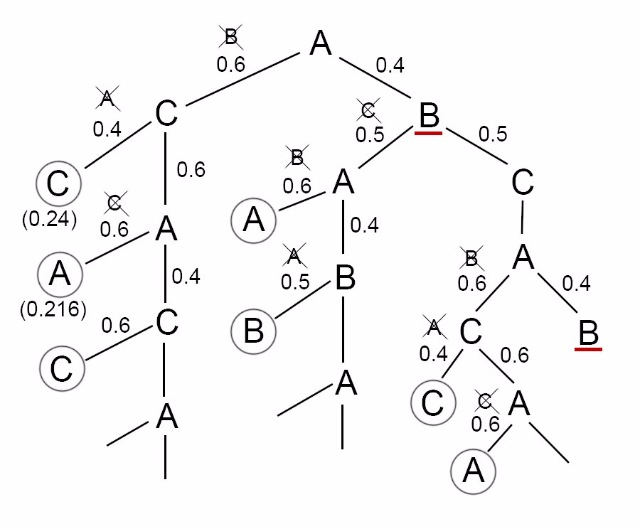
\includegraphics[width=10cm]{images/truel_task37.jpg}
\end{figure*}
\begin{enumerate}
\item Если первым выстрелом А убил В (с вероятностью 0.6),
то шанс победить остается у А и у С. Вероятность,
что дальше С попадет в цель своим первым выстрелом и победит = 0.24.
Если же С промахивается, а следующим ходом А его убивает,
то А побеждает с вероятностью 0.216. Если А промахивается,
то исход дуэли решает С и цикл повторяется. Можно заметить,
что вероятность победы любого из них —
сумма бесконечно убывающей геометрической прогресии.

$\P(\text{победа C})= \frac{0.24}{1-0.24} = 0.32$

$\P(\text{победа A}) = \frac{0.216}{1-0.24} = 0.28$
\item Если первым выстрелом А не убивает В, то

а) следующим ходом В убивает С и победа разыгрывается между А и В;

б) В не убивает С, тогда (С стреляет в воздух) либо А убивает В, либо промахивается,
и ход опять падает на В (при этом все живы) — цикл повторяется.

а) $\P(\text{победа A}) = \frac{0.12}{1-0.2} = 0.15$

$\P(\text{победа B}) = \frac{0.04}{1-0.2} = 0.05$

б) Теперь можно учесть повтор цикла для вероятности А и В (случай,
когда А промахнулся и ход опять перешел В)

$\P(\text{победа A}) = \frac{0.15}{1-0.2} = 0.19$

$\P(\text{победа B}) = \frac{0.05}{1-0.2} = 0.06$

Если же А сразу убивает В, то (учитывая все циклы)

$\P(\text{победа A}) = \frac{\frac{0.0432}{1-0.24}}{1-0.2} = 0.07$

$\P(\text{победа C}) = \frac{\frac{0.048}{1-0.24}}{1-0.2} = 0.08$

\textbf{Проверим сумму вероятностей}: $0.32 + 0.28 + 0.19 + 0.06 + 0.07 + 0.08 = 1$

\textbf{Результат}:

$\P(\text{победит A}) = 0.28 + 0.19 +0.07 = 0.54$

$\P(\text{победит B}) = 0.06$

$\P(\text{победит С}) = 0.32 + 0.08 = 0.4$
\end{enumerate}
\end{sol}

\end{problem}


\begin{problem}
Игра Паррондо

В игре $A$ ты с вероятностью $0.49$ выигрываешь один рубль
и с вероятностью $0.51$ проигрываешь один рубль.

Игра $B$ чуть более хитрая. Если сумма в твоём кошельке делится на три,
то ты выигрываешь один рубль с вероятностью $0.1$ и проигрываешь один рубль
с вероятностью $0.9$. Если же сумма в твоем кошельке не делится на три,
то ты выигрываешь один рубль с вероятностью $0.74$
и проигрываешь один рубль с вероятностью $0.26$.

Изначально у тебя в кошельке 100 рублей. Что произойдёт с твоим благосостоянием,
если:

\begin{enumerate}
\item Ты будешь бесконечное количество раз играть в игру $A$?
\item Ты будешь бесконечное количество раз играть в игру $B$?
\item Ты будешь бесконечное количество раз
равновероятно выбирать игру $A$ или игру $B$?
\end{enumerate}

\begin{sol}
Если играть в игру $A$, то благосостояние будет стремиться к нулю.
Если играть в игру $B$, то благосостояние будет стремиться к нулю.
Если равновероятно играть в игры $A$ и $B$, то благосостояние
будет стремиться к бесконечности.
\end{sol}

\end{problem}


\begin{problem}
Во время Второй Мировой войны американские военные собрали статистику попаданий пуль в фюзеляж самолёта.  По самолётам, вернувшимся из полёта на базу, была составлена карта повреждений среднестатистического самолёта. С этими данными военные обратились к статистику Абрахаму Вальду с вопросом, в каких местах следует увеличить броню самолёта.

Что посоветовал Абрахам Вальд и почему?

\begin{sol}
На базу будут возвращаться только самолёты, имеющие некритичные повреждения. Поэтому чем больше попаданий в какое-то место самолёта, тем менее данное место важно для живучести самолёта. Абрахам Вальд посоветовал укреплять те места, где не было попаданий.
\end{sol}

\end{problem}


\begin{problem}
Задача о немецких танках
\marginnote{Незадолго до высадки союзников в Нормандии, 6 июня 1944 года, в распоряжении союзников было всего два (!) немецких танка «Пантера V». По серийным номерам на шасси танков союзники оценили выпуск в феврале 1944 в 270 танков. Фактический выпуск «Пантер V» согласно немецким документам в феврале 1944 составил 276 танков, \autocite{ruggles1947empirical}. }

Предположим, что все выпущенные танки имеют порядковый номер. От самого первого выпущенного танка, имеющего номер $1$, до самого последнего танка, имеющего номер $n$. В бою удалось подбить танки с номерами $15$, $29$ и $23$.

\begin{enumerate}
\item Постройте оценку количества танков методом моментов;
\item Постройте оценку количества танков методом максимального правдоподобия;
\item Постройте несмещенную оценку количества танков с наименьшей дисперсией.
\end{enumerate}

\begin{sol}
Оценка метода моментов:
\[
\hat{n}_{MM}=2\bar{X}-1
\]
Оценка максимального правдоподобия:
\[
\hat{n}_{ML}=\max\{X_1,X_2, \ldots, X_k\}
\]

\end{sol}

\end{problem}


\begin{problem}
Саша и Маша хорошо перетасовали колоду в 52 карты и удалили из неё все онёры («картинки»),
так что остались одни фоски (числовые карты). Саша выбирает одну из первых 10 карт наугад.
Узнав значение этой карты, он открывает соответствующую следующую по счёту карту.
Открыв новую карту и руководствуясь её значением,
Саша открывает еще одну новую карту и т.д. до тех пор, пока хватает колоды.

Не перемешивая колоду Маша повторяет Сашин алгоритм действий.
С помощью симуляций определите, какова примерно вероятность того,
что Саша и Маша остановятся на одной карте.

\begin{sol}
\end{sol}

\end{problem}


\begin{problem}
Парчовую ленту длиной 1 км разрезают в $(n-1)$-ом случайно равномерно распределенном месте,
чтобы поделить её на $n$ принцесс.
Скромнице Василисе достаётся самый короткий кусочек ленты.

\begin{enumerate}
\item Какова ожидаемая длина Василисиного куска?
\item Какова ожидаемая длина самого короткого кусочка кроме Василисиного?
\end{enumerate}

\begin{sol}
Найдём вероятность того, что минимальная длина больше $d$.
Представим себе большую колоду из $N$ карт, в которой $(n-1)$ отмеченная карта.
Нам нужна вероятность того,
что при вытягивании карт по очереди между ними будет минимум $dN$ карт.
Однако при вытягивании меченой карты, можно следующие $dN$ карт вытягивать с конца колоды.
Это не повлияет на случайность порядка, а вероятность будет считать проще.
Нам нужна фактически вероятность того,
что в конце колоды будет $(n-1)dN$ немеченных карт и $dN$ немеченных карт в начале колоды.


В случае $k$-го по счёту минимального куска:
\[
\frac{1}{n}\left( \frac{1}{n} + \ldots + \frac{1}{k}\right)
\]

Идея доказательства:
\[
\E(X) + \frac{1-n\E(X)}{(n-1)^2}=\ldots=
\frac{1}{n}\left( \frac{1}{n} + \frac{1}{n-1}\right)
\]
\end{sol}


\end{problem}


\begin{problem}
Роковая дама играет в азартную игру. Перед дамой хорошо перетасованная колода в 52 карты.
Дама открывает карты одну за одной. В любой момент дама может
сделать пророчество «Следующая карта будет дамой».
Если пророчество сбывается, то дама получает 100 рублей.

\begin{enumerate}
\item Какова оптимальная стратегия дамы?
\item Какова вероятность выигрыша при использовании оптимальной стратегии?
\end{enumerate}

\begin{sol}
Вместо того, чтобы делать ставку на следующую карту, можно делать ставку на последнюю карту,
т.к. информация о них одинаковая. А для последней карты не важно,
когда делать пророчество, поэтому все стратегии приносят вероятность выигрыша $4/52$.
\end{sol}

\end{problem}


\begin{problem}
Ветреная Машенька пишет романтические смс Андрею и Борису.
Первое смс она пишет Андрею, второе — Борису и третье — Борису.
Далее каждое следующее смс она пишет Андрею с вероятностью равной доле ранее отправленных Андрею смс.
Всего за день Машенька отправила 100 смс.

\begin{enumerate}
\item Какова вероятность того, что четвёртое смс она напишет Борису?
\item Какова вероятность того, что 100-ое смс она напишет Борису?
\item Какова вероятность того, что последние три смс она напишет Борису?
\item Сколько в среднем смс она напишет Борису?
\item Какова вероятность того, что ровно 20 смс она напишет Борису?
\item Какова вероятность того, что ровно $k$ смс она напишет Борису?
\item Машенька продолжает писать смс Андрею и Борису, не остановившись на $n=100$. Она загадала, что если тысячу раз подряд напишет смс Борису, то выйдет за него замуж. Какова вероятность, того, что Машенька выйдет замуж за Бориса? Сколько в среднем смс всего до замужества она напишет?
\end{enumerate}

\begin{sol}
\begin{enumerate}
\item
\[
X_n =\left\{\begin{array}{l} {1,\quad n\text{-я смс отправлена Борису (это же успех!)}} \\ {0,\text{ иначе}} \end{array}\right.
\]

Т.к. вероятность написания смс Андрею равна доле предыдущих смс Андрею, то вероятность написания смс Борису равняется доле предыдущих смс, адресованных ему.

$\P(X_4=1) = \frac{2}{3}$
\item $\P(X_5=1) = \frac{2}{3}\cdot\frac{3}{4}+\frac{1}{3}\cdot\frac{2}{4} = C_{1}^{0}\cdot(\frac{2}{3})^{1}\cdot(\frac{1}{3})^0\cdot\frac{3}{4}+C_{1}^{1}\cdot(\frac{2}{3})^{0}\cdot(\frac{1}{3})^1\cdot\frac{2}{4}=\frac{2}{3}$

$\P(X_6=1) = (\frac{2}{3})^2\cdot\frac{4}{5}+\frac{2}{3}\cdot\frac{1}{3}\cdot\frac{3}{5}\cdot 2 + (\frac{1}{3})^2\cdot\frac{2}{5} = \frac{3}{2} = C_{2}^{0}\cdot(\frac{2}{3})^{2}\cdot(\frac{1}{3})^0\cdot\frac{4}{5}+C_{2}^{1}\cdot(\frac{2}{3})^{1}\cdot(\frac{1}{3})^1\cdot\frac{3}{5}+C_{2}^{2}\cdot(\frac{2}{3})^{0}\cdot(\frac{1}{3})^{2}\cdot\frac{2}{5} = \frac{2}{3} $

\ldots

$\P(X_n=1) = \sum_{i=0}^{n-4} C_{n-4}^{i}\cdot(\frac{2}{3})^{n-4-i}\cdot(\frac{1}{3})^i\cdot\frac{n-2-i}{n-1} = \frac{2}{3}$

$\P(X_{100}=1) = \sum_{i=0}^{96} C_{96}^{i}\cdot(\frac{2}{3})^{96-i}\cdot(\frac{1}{3})^i\cdot\frac{98-i}{99} = \frac{2}{3}$
\item Здесь важно учесть, что тот факт, что предыдущее смс написано Борису, будет влиять на вероятность следующего

$\P(X_{98},X_{99},X_{100}=1) = \frac{2}{3}\cdot\frac{97\cdot\frac{2}{3}+1}{98}\cdot\frac{97\cdot\frac{2}{3}+2}{99}\approx 0.29$
\item $\E(X_1, X_2, \ldots  , X_{100}) = \E(X_1)+ \E(X_2) + \ldots  + \E(X_{100}) = 100\cdot 1 \cdot \frac{2}{3} = \frac{200}{3}$
\item $\P( \sum_2^{21}X_n >= 20) = 1\cdot1\cdot\frac{2}{3}\cdot \frac{3}{4}\cdot \frac{4}{5}\cdot \frac{5}{6}\cdot\ldots \cdot \frac{19}{20}$

$\P( \sum_1^{100}X_n = 20) = C_{97}^{18}\cdot1\cdot1\cdot\frac{2}{3}\cdot \frac{3}{4}\cdot \frac{4}{5}\cdot \frac{5}{6}\cdot\ldots \cdot \frac{19}{20} \cdot \frac {1}{21}\cdot \ldots  \cdot \frac{79}{99}= C_{97}^{18}\cdot\frac{19!\cdot79!}{99!}=\frac{19!\cdot79!\cdot97!}{99!\cdot18!\cdot79!}=\frac{19}{98\cdot99}=\frac{19}{9702}\approx 0.002$
\item $\P( \sum_1^{100}X_n = k) = C_{97}^{k-2}\cdot \frac{(k-1)!\cdot(100-k-1)!}{99!} = \frac{(k-1)!\cdot(99-k)!\cdot97!}{99!\cdot(99-k)!\cdot(k-2)!}=\frac{k-1}{9702}$
\item $\P(\sum_m^{m+999}X_n=1000) = 1\cdot1\cdot\frac{2}{3}\cdot\frac{3}{4}\cdot\ldots \cdot\frac{998}{999}\cdot\frac{999}{1000}=\frac{1}{500}$

Маловато для замужества\ldots
\end{enumerate}
\end{sol}

\end{problem}


\begin{problem}
Злобный Дракон поймал принцесс Настю и Сашу и посадил в разные башни. Перед каждой из принцесс Злобный Дракон подбрасывает один раз правильную монетку. А дальше даёт каждой из них шанс угадать, как выпала монетка у её подруги. Если хотя бы одна из принцесс угадает, то Злобный Дракон отпустит принцесс на волю. Если обе принцессы ошибутся, то они навсегда останутся у него в заточении.

Подобная практика у Злобного Дракона исследователями была отмечена уже давно, поэтому принцессы имели достаточно времени договориться на случай вероятного похищения.

Как следует поступать принцессам при подобных похищениях?

\begin{sol}
Настя может угадывать в случае, если монетки выпали одинаково, а Саша — если по-разному.
\end{sol}


\end{problem}


\begin{problem}
Удав Анатолий любит французские багеты. Длина французского багета равна 1 метру. За один заглот Удав Анатолий заглатывает кусок случайной длины равномерно распределенной на отрезке $[0;1]$. Для того, чтобы съесть весь багет удаву потребуется случайное количество $N$ заглотов.
\begin{enumerate}
\item Найдите $\E(N)$ и $\Var(N)$
\item Как поменяются ответы, если багет имеет длину 2 метра?
\end{enumerate}

\begin{figure*}
  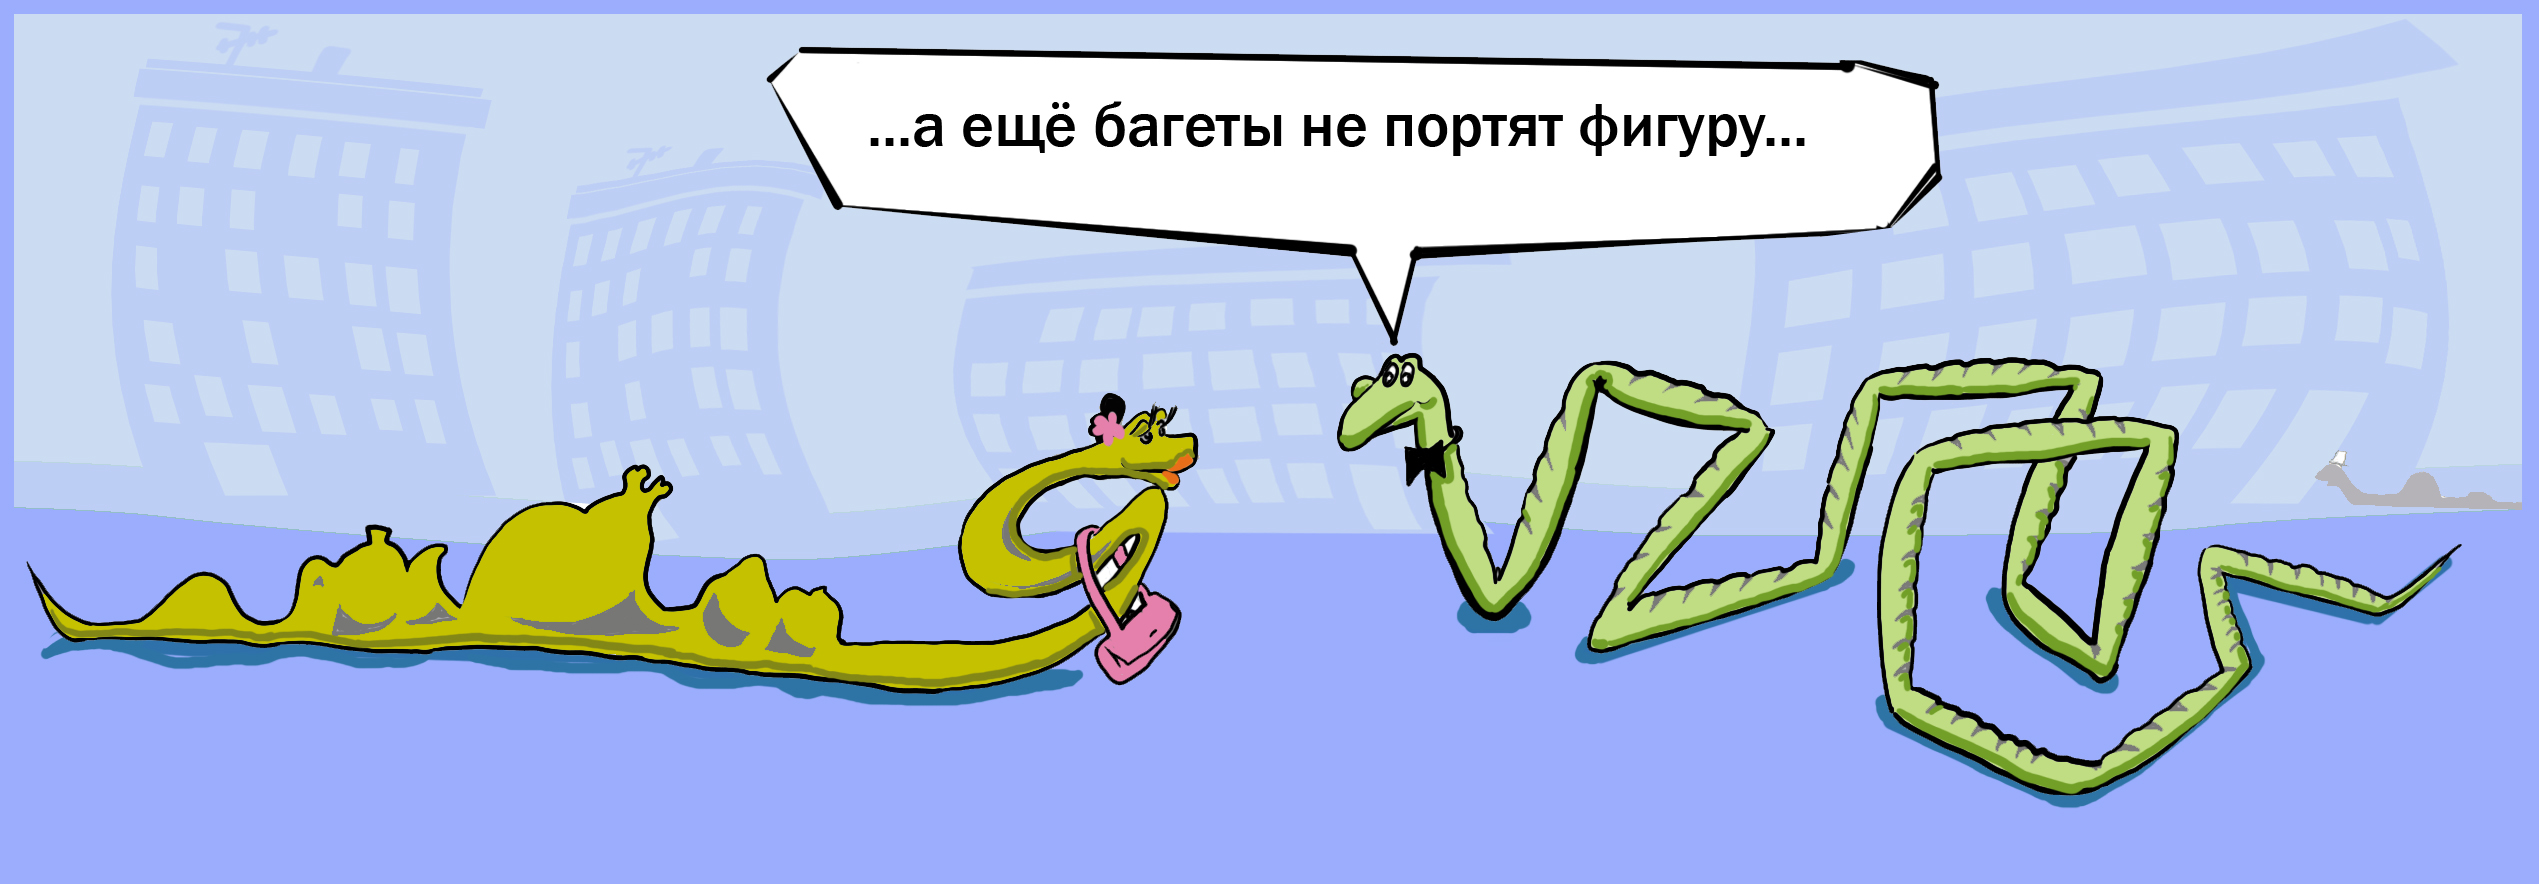
\includegraphics[width=17cm]{images/python_anatoliy.jpg}
  \caption{Удав Анатолий и Гюрза Леопольдина}
\end{figure*}


\begin{sol}
$\E(N)=e$.

Заметим, что верно следующее соотношение
\[
\min \{n : X_1 + X_2 + \ldots \geq 1 \} = \sum_{i = 1}^{\infty} \I \{\sum_{k = 1}^i X_k < 1\} + 1
\]
В правой части мы будем суммировать единицы пока сумма случайных величин меньше 1 и потом прибавляем один, чтобы учесть $n$, на котором сумма перепрыгнет единицу. Математическое ожидание суммы — это сумма математических ожиданий. Математическое ожидание индикатора — это вероятность. Получаем:
\[
\E(n) =  \sum_{i = 1}^{\infty} \P (S_i < 1) + 1
\]
Посчитаем такие вероятности. Для случая $i = 1$ вероятность равна 1. При $i = 2$ мы можем нарисовать квадрат соответствующий совместному распределению $X_1$ и $X_2$. Плоскость $X_1 + X_2 < 1$ отсекает половину площади, значит вероятность равна $1/2$.

Как посчитать все остальные вероятности? Рассмотрим $S_n$. Совместному распределению $n$ равномерных случайных величин соответствует $n$-мерный куб. Плоскость $\sum X_i = 1$ проходит через все точки типа: $(1, 0, \ldots, 0), (0, 1, \ldots, 0)$. Посчитаем объём фигуры, которая образована такой плоскостью и точкой $(0, 0, \ldots, 0)$ — это и будет искомая вероятность. Воспользуемся формулой объёма $n$-мерной пирамиды: $V = \frac{1}{n}SH$. В качестве вершины возьмём точку $(1,0,\ldots)$. Заметим, что расстояние от неё до плоскости $x_1 = 0$ в которой лежат остальные точки равно 1.

Площадь основания, это объём такой же фигуры, только образованной $n-1$ точкой. Получаем соотношение:
\[
\P (S_n < 1) = \frac{1}{n} \P (S_{n-1} < 1)
\]
Тогда искомый ряд равен:
\[
\E(N) = \sum_{i= 1}^{\infty} \frac{1}{i!} + 1
\]
Его сумма равна $e$, как ряд Маклорена для $e^x$.


Ещё решение. Рассмотрим багет длины $x<1$. Заметим формулу для вероятности,
\[
\P(X=n) = \P(x_{1} +\ldots+x_{n-1}\le x) - \P(x_{1}+\ldots+x_{n}\le x)
\]

По индукции можем показать, что $\P(x_{1}+\ldots+x_{n}\le x)=\frac{x^n}{n!}$

Поэтому
\[
\P(X=n)=\frac{x^{n-1}}{(n-1)!}-\frac{x^n}{n!}
\]

Далее можно решать через ряд Тейлора:

\[
\E(N)=e^x, \Var(N)=e^x(1+2x)-e^{2x}
\]

И ещё решение:

Пусть сейчас Удав уже съел суммарно багетов на $a<1$ метров. Обозначим $N(a)$ — число оставшихся шагов до съедения $x$ метров. Введём две функции $f(a)=\E(N(a))$ и $g(a)=\E(N^{2}(a))$.

Методом первого шага можно получить уравнения:
\[
\begin{cases}
f(a)=\int_{a}^{x}f(t)dt \\
g(a)=1+\int_{a}^{x}g(t)dt+2\int_{a}^{x}f(t)dt
\end{cases}
\]

И начальные условия $f(x)=g(x)=1$ Далее дифференциируем и получаем решаемые дифференциальные уравнения.

\end{sol}


\end{problem}


\begin{problem}
Жозеф Луи Франсуа Бертран подкидывает правильную монетку $n$ раз. Пафнутий Львович Чебышёв\footnote{Да, да, предпоследняя буква в окончании именно «ё»} подкидывает правильную монетку $(n+1)$ раз. Какова вероятность того, что у Пафнутия Львовича выпадет больше «орлов», чем у Жозефа Луи Франсуа?

\begin{sol}
Допустим, что после $n$ подбрасываний Пафнутий лидирует с вероятностью $p$. Тогда в силу симметрии задачи, вероятность равенства числа «орлов» после $n$ подбрасываний равна $1-2p$. Следовательно, вероятность победы Пафнутия равна $p+(1-2p)\frac{1}{2}=\frac{1}{2}$.
\end{sol}

\end{problem}


\begin{problem}
Сломанный пульт

Роберт Адлер нажимает на кнопку «Вкл/Выкл» на пульте дистанционного управления телевизором. Изначально телевизор включён. Батарейки у пульта сели, поэтому в первый раз кнопка срабатывает с вероятностью $1/2$. Далее вероятность срабатывания кнопки падает. Какова вероятность, что после 100 нажатий телевизор окажется включён?


\begin{sol}
Можно попробовать посчитать вероятности для нескольких первых нажатий и по индукции получить ответ $1/2$.
\end{sol}

\end{problem}


\begin{problem}
Киллер

Правила игры «Киллер» просты. Игроки пишут на бумажках, как их зовут, и кладут бумажки в шляпу. Каждый тянет из шляпы имя своей первой жертвы. Если первой жертвой игрока является он сам, то он совершает «самоубийство» и дальше не играет\footnote{В некоторых вариантах правил, если игрок вытянул из шляпы своё имя, то он должен вытянуть другую бумажку.}. Чтобы убить жертву, надо остаться с ней наедине и сказать: «Ты убит!». Убийца забирает себе все бумажки, набранные убитым, и начинается охотиться за тем, за кем охотился убитый.  Побеждает тот, кто наберёт больше всех бумажек к концу игры. Заметим, что в «Киллере» каждый игрок оказывается втянут в одну из нескольких цепочек.

В «Киллера» играют 30 человек, из них 20 девушек.

\begin{enumerate}
\item Какова вероятность того, что в цепочке, начинающейся с Маши Сидоровой ровно 5 человек?
\item Какова вероятность того, что в цепочке, начинающейся с Маши Сидоровой ровно 5 девушек?
\item Какова вероятность того, что все девушки попадают в одну цепочку убийц и жертв?
\item Какова вероятность того, что все игроки попадают в общую цепочку?
\item Сколько в среднем цепочек в «Киллере»?
\item Сколько в среднем «самоубийц»?
\item Рассмотрим вариант, в котором нет самоубийств, то есть раздача бумажек организована так, что ни один игрок не может получить свою бумажку при раздаче. Как изменятся ответы?
\end{enumerate}

\begin{sol}

\begin{enumerate}
\item
\[
\P(\text{ровно 5 человек}) = \frac{29}{30} \frac{28}{29} \frac{27}{28} \frac{26}{27} \frac{1}{26} = \frac{1}{30}
\]
\item Желаемая цепочка обязательно имеет вид: Маша — Парни — Девушка — Парни — Девушка\ldots Каждый блок из парней может иметь нулевую длину. Нам полностью безразлично, что происходит в блоках из парней, нам важно лишь, чтобы при выходе из блока парней жертвой была новая девушка. Поэтому мы и перемножаем только вероятности для выбора девушек:
\[
\P(\text{ровно 5 девушек}) = \frac{19}{20} \frac{18}{19} \frac{17}{18} \frac{16}{17} \frac{1}{16} = \frac{1}{20}
\]
\end{enumerate}

Вариация без самоубийц
\begin{enumerate}
\item
\[
\P(\text{ровно 5 человек}) = 1 \cdot \frac{28}{29} \frac{27}{28} \frac{26}{27} \frac{1}{26} = \frac{1}{29}
\]
\end{enumerate}


\end{sol}

\end{problem}


\begin{problem}
Ной Палмер Чепмэн\footnote{почтмейстер из Канастоты, вероятно, изобретатель игры «пятнашки»} рассыпал фишки для игры в пятнашки и расставляет их на поле в случайном порядке. Какова вероятность того, что он сможет решить получившуюся головоломку?

\begin{sol}
Легко экспериментально установить, что все фишки кроме двух последних можно поставить на свои места. Например, сначала выставляются $1$--$4$, затем $5$--$8$, затем $9$, $13$ и всё оставшееся кроме $14$ и $15$.  Один вариант не сводится к другому, так как любое движение в пятнашках не изменяет четность перестановки. Чётных и нечётных перестановок одинаковое количество, поэтому вероятность равна $1/2$.
\end{sol}

\end{problem}


\begin{problem}
Задача о 100 заключенных

У ста узников тюрьмы есть последний шанс на спасение. В комнате стоит шкаф в котором сто занумерованных ящичков. Палач кладёт в каждый ящичек бумажку с номером ровно одного из заключенных в случайном порядке и задвигает все ящички. Узники заходят в комнату один за другим. Каждый узник может открыть любые 50 ящичков. После каждого узника все ящички задвигаются в исходное положение. Если каждый узник находит свой номер, то все узники будут помилованы. Если хотя бы один из узников не найдёт свой номер, то все будут казнены.

Узники могут предварительно договориться о стратегии.

\begin{enumerate}
\item Какова оптимальная стратегия?
\item Какую вероятность выигрыша она обеспечивает?
\end{enumerate}

\begin{sol}
Открыть ящичек со своим номером, далее открывать ящички с номером, написанным на вытащенной бумажке. Вероятность выигрыша, $1-(H_{100}-H_{50}) \approx 1- \ln 2$, где $H_n$ — гармоническое число, $H_n=1+\frac{1}{2} + \frac{1}{3} + \ldots + \frac{1}{n}$.
\end{sol}

\end{problem}


\begin{problem}
Андрей Абрикосов, Борис Бананов и Вова Виноградов играют одной командой в игру.
В комнате три закрытых внешне неотличимых коробки: с абрикосами, бананами и виноградом.
Общаться после начала игры они не могут, но могут заранее договориться о стратегии.
Они заходят в комнату по очереди. Каждый из них может открыть две коробки по своему выбору.
Перед следующим игроком коробки закрываются. Если Андрей откроет коробку абрикосами,
Борис — с бананами, а Вова — с виноградом, то они выигрывают.
Если хотя бы один из игроков не найдёт свой фрукт, то их команда проигрывает.

\begin{enumerate}
\item Какова оптимальная стратегия?

\item Какова вероятность выигрыша при использовании оптимальной стратегии?
\end{enumerate}


\begin{sol}
$2/3$
\end{sol}

\end{problem}


\begin{problem}
Дед Мороз развешивает новогодние гирлянды. Аллея состоит из 1000 елок. Каждой гирляндой Дед Мороз соединяет две елки (не обязательно соседние). В результате Дед Мороз повесил 500 гирлянды и все елки оказались украшенными. Какова вероятность того, что существует хотя бы одна гирлянда, пересекающаяся с каждой из других?

Например, гирлянда 5-123 (гирлянда соединяющая 5-ую и 123-ю елки) пересекает гирлянду 37-78 и гирлянду 110-318.

\begin{sol}
Решение номер раз!

1) Всего получилось $n=500$ пар ёлок, поэтому выбираем из $2n=1000$ ёлок.Пронумеруем ёлки от $1$ до $2n$.

2) Будем поочерёдно выбирать пары ёлок. Тогда, если нам известны $2j$ выбранных ёлок, мы можем выбрать $(2j+1)$ ёлку из $(2n-2j)$ оставшихся, назвать её $A_{j+1}$ и найти ей пару среди оставшихся $2n-(2j+1)$ ёлок. Лучше выбирать $A_j$ ближе к центру, чтобы количество ёлок было максимально сбалансировано между двух сторон: с левой стороны ${1,\ldots ,n}$ и с правой стороны ${n+1,\ldots ,2n}$.

3) Первый шаг. Начинаем с $A_1=n$ и $B_1$ её пары. Предполагая, что мы знаем $A_1,\ldots ,A_j$  и соответствующие им $B_1,\ldots , B_j$ и выбирем $A_{j+1}$ ёлку следующим образом:

– если $B_j$ ёлка стоит на левой стороне, то пусть $A_{j+1}$ ёлка будет самой левой с правой стороны;

– если $B_j$ ёлка стоит на правой стороне, то пусть $A_{j+1}$ ёлка будет самой правой с левой стороны

Замечание: $A_j<B_j$, точно тогда, когда $B_j$ справа.

4) Второй шаг. Выбор $B_{j+1}$ (пары для $A_{j+1}$) из оставшихся $2n-(2j+1)$ оставшихся.

5) Назовём $j$-ую пару ёлок парой AB-типа, если $A_j<B_j$.
Назовём $j$-ую пару ёлок парой BA-типа, если $A_j>B_j$.

Теперь левая и правая сторона аллеи имеют одинаковое количество пар ёлок AB-типов. После первого BA-типа, левая сторона имеет на две соединённых ёлки больше. Этот дисбаланс по двум ёлкам одновременно поддерживается, пока не закончатся БА-типы, до следующего AB-типа, восстанавливающего баланс. Отметим, что не существует непарных ёлок между крайней левой и крайней правой точкой $A_1,\ldots ,A_j$.

6) После выбора $(n-2)$-ой пары, остаётся 4 ёлки с номерами $a < b < c < d$. Имеем два варианта:

– сбалансированный случай: $a$ и $b$ на левой стороне, $c$ и $d$ на правой стороне.

– несбалансированный случай: $a$ на левой стороне, $b$, $c$ и $d$ на правой стороне.

7) Сбалансированный случай (всего три варианта для соединения с ёлкой $а$):

Сейчас все $A_{j, j} \leq n-2$ должны быть между $a$ и $c$, так как они не соединены гирляндой, и $a$ слева, и $c$ справа.

Если ёлку $a$ соединить с ёлкой $c$, то соединяющая их гирлянда пересечёт все оставшиеся гирлянды. Аналогично для гирлянды, соединяющей ёлки $a$ и $d$.

Докажем, что пара $a$ и $b$ не пересечет все остальные.

Действительно, пара $a,b$ не сможет пересечь пару $c,d$, так как они разделены и не имеют общих точек. Предположим, что существует гирлянда, соединяющая $A_{j_0}$ и $B_{j_0}$ ёлки (для $j\leq n-2$) и пересекающая все остальные гилянды. В сбалансированном случае все $A_{j, j} \leq n-2$ должны лежать между $b$ и $c$, поэтому гирлянда $A_{0j};B_{0j}$ не пересечёт обе гирлянды $[a,b]$ и $[c,d]$.

Таким образом, получаем вероятность того, что хотя бы одна гирлянда пересечёт все остальные равна $2/3$.

8) Несбалансированный случай
$(n-2)$-ая пара должна быть ВА-типа. С другой стороны, горлянда $А_{j0},B_{j0}$ пересекает гирлянду $[c,d]$, и поэтому пара $j_0$ должна быть АВ-типа. Так, существует $k \in [j0 + 1, n − 2]$, такое что $(k − 1)$-ая пара AB-типа, когда $k$-ая пара BA-типа. В частности, $A_k < n$ (всегда при $k> 1$ и предыдущей паре AB-типа) and $A_k < A_{j0}$ (при $k > j_0$ и предыдущей паре АВ-типа). Это означает, что $[B_k, A_k] \cap [A_{j0}, B_{j0}]=\emptyset$. Противоречие, ни одна гирлянда не пересекает все оставшиеся в этом случае.

Ответ: $2/3$, \autocite{gravner20problems}

Решение номер два!

Докажем следующее утверждение.

Утверждение. Бросим $2n \geq 4$ точек $X_1, X_2, \ldots, X_{2n}$ случайным образом на отрезок $[0;1]$. Пусть для $1 \leq i \leq n$ $J_i$ — это отрезок с концами $X_{2i-1}$ и $X_{2i}$.
Тогда вероятность того, что найдётся такой отрезок $J_i$, который пересекает все другие отрезки, равна $2/3$ и не зависит от $n$.

Доказательство. Бросим $2n+1$ точек на окружность, тогда $2n$ точек образуют пары, а оставшуюся обозначим $X$ и будем считать её и началом, и концом отрезка.
Каждому получившемуся отрезку присвоим уникальное имя.
Далее, будем двигаться от точки $X$ по часовой стрелке до тех пор, пока не встретим одно и то же имя дважды, например «а».
После этого пойдём в обратную сторону, и будем идти, пока не встретим какое-нибудь другое имя дважды, например, «б».
Теперь посмотрим на получившуюся последовательность между «б» и «а» на концах пути, читая её по часовой стрелке от «б» до «а».
Нас интересует взаимное расположение $X$, второй «а» и второй «б».
Зная, что «а» стоит после $X$, выпишем все возможные случаи, где может стоять «б»:
\begin{enumerate}
\item перед $X$
\item между $X$ и «а»
\item после «а»
\end{enumerate}
Покажем, что во втором и третьем случае отрезок «б» пересекает все остальные, а в первом такого отрезка вообще нет. Попутно заметим, что появление каждого и случаев равновероятно.

Действительно, если «б» стоит после $X$, и отрезок соответствующий этому имени, не пересекает какой-нибудь другой отрезок «в», то последовательность выглядела бы как «бвв$X$б» или «б$X$ввб», что противоречит описанному построению.
Если «б» стоит перед $X$ и отрезок «в» пересекает оба отрезка «а» и «б», то мы снова приходим в противоречие с построением.
В итоге, получаем, что искомая вероятность равна $2/3$.
\end{sol}
\end{problem}


\begin{problem}
Птички на проводе

На телеграфный провод равномерно и независимо друг от друга садятся случайным образом  $n$ птичек. Число птичек очень велико. Маляр-электрик Степан Грибоедов красит белой краской отрезок провода от каждой птички до ближайшей. Каждый участок провода оказывается в результате либо ни разу не покрашенным, либо покрашенным один, либо два раза.

Найдите среднюю длину непокрашенной части провода, части, покрашенной один раз, и части, покрашенной два раза.

\begin{sol}
\url{http://www.cut-the-knot.org/Curriculum/Probability/BOW4.shtml}
\url{http://math.stackexchange.com/questions/227990/}
$2/18$, $5/18$, $11/18$
\end{sol}

\end{problem}


\begin{problem}
В углу шахматный доски стоит конь. Мы перемещаем коня наугад, выбирая каждый допустимый ход равновероятно. Сколько в среднем пройдет ходов прежде чем он вернется в исходную клетку?

\begin{sol}
Шаг 1. Находим стабильное распределение для Марковского процесса. Марковскую цепь можно представить в виде графа, в котором вершины — это состояния процесса, а ребра — переходы между состояниями, и на ребре из $i$ в $j$ написана вероятность перехода из $i$ в $j$.
Мы видим, что этот процесс устойчив, если масса для каждого квадрата шахматной доски будет пропорциональна числу ходов коней, ведущих от него. Иными словами, каждый квадрат доски с $n$ шагами, исходящими из него, будет иметь массу n движущихся к нему и массу n движущихся от него, так что всё уравновешивается.

Шаг 2. Нам нужно найти массу всей системы, что есть сумма всех возможных передвижений коня. Для данной шахматной фигуры есть $8$ возможных направлений и каждое может иметь исходить из квадрата $6 \times 7$, так что масса распределения равна $336$.

Шаг 3. Поскольку масса угловой клетки равна двум, она представляет собой $\frac{2}{336} = \frac{1}{168}$ всей массы распределения. Поскольку процесс рекуррентный, блуждание от любого квадрата будет в этом конкретном углу $\frac{1}{168}$ от всех ходов. Это означает, что в среднем конь пройдёт $168$ ходов, прежде чем он вернётся в исходную клетку.

Ответ: $168$
\end{sol}


\end{problem}


\begin{problem}
Китайский ресторан

Каждую минуту в китайский ресторан приходит новый посетитель.
Если в ресторане сидит $n$ человек, а за конкретным столиком сидит $b$ человек,
то вероятность того, что новый посетитель присоединится к этому столику равна $\frac{b}{n+\theta}$.
С вероятностью $\frac{\theta}{n+\theta}$ посетитель сядет за отдельный столик.

Каково ожидаемое число занятых столиков через $t$ минут после открытия?

\begin{sol}
Идея решения состоит в том, что для подсчёта матожидания количества занятых столиков в момент времени $t$ мы будем отталкиваться от данных в момент времени $t-1$. К моменту времени $t$, пока ещё не зашёл посетитель, количество уже занятых столов является случайной величиной, принимающей значения от 1 до $t-1$ с определёнными вероятностями. Далее количество занятых столиков либо возрастает на 1 с известной вероятностью либо остаётся неизменным.

$\E(k_1)=1$, что очевидно. Человек приходит и с вероятностью 1 садится за отдельный стол.

$\E(k_2)=1\cdot \frac{1}{\theta+1}+2\cdot\frac{\theta}{\theta+1}$, так как с вероятностью $\frac{1}{\theta+1}$ человек присоединится к занятому столику, иначе сядет за второй стол.

$\E(k_3)=\frac{1}{\theta+1}\left(1\cdot \frac{2}{\theta+2}+2\cdot\frac{\theta}{\theta+2}\right)+\frac{\theta}{\theta+1}\left( 2\cdot\frac{2}{\theta+2}+3\cdot\frac{\theta}{\theta+2}\right)=$

$=1\cdot\frac{2!}{(\theta+1)(\theta+2)}+2\cdot 3\frac{\theta}{(\theta+1)(\theta+2)}+3\cdot\frac{\theta^2}{(\theta+1)(\theta+2)}$

$~$

\begin{multline*}
\E(k_4)=\frac{2!}{(\theta+1)(\theta+2)}\left( 1\cdot\frac{3}{\theta+3}+2\cdot\frac{\theta}{\theta+3} \right)+3\frac{\theta}{(\theta+1)(\theta+2)}\cdot \\
\cdot \left( 2\cdot\frac{3}{\theta+3}+3\cdot\frac{\theta}{\theta+3} \right)+\frac{\theta^2}{(\theta+1)(\theta+2)}\left( 3\cdot\frac{3}{\theta+3}+4\cdot\frac{\theta}{\theta+3} \right)=\\
=1\cdot\left( \frac{3!}{(\theta+1)(\theta+2)(\theta+3)} \right)+2\cdot\left( \frac{11\theta}{(\theta+1)(\theta+2)(\theta+3)} \right)+\\
+3\cdot\left( \frac{6\theta^2}{(\theta+1)(\theta+2)(\theta+3)} \right)+4\cdot\left( \frac{\theta^3}{(\theta+1)(\theta+2)(\theta+3)} \right)
\end{multline*}

Что мы имеем?

\[
\E(k_t)=\sum_{j=1}^t j\cdot a_{tj}\cdot \frac{\theta^{j-1}}{(\theta+1)(\theta+2)\dots(\theta+t-1)}
\]
где $j$ – число занятых столов, $a_{tj}\cdot \frac{\theta^{j-1}}{(\theta+1)(\theta+2)\dots(\theta+t-1)}$ – вероятность того, что именно такое количество столов будет занято. Понятно, откуда берётся дробь
\[
\frac{\theta^{j-1}}{(\theta+1)(\theta+2)\dots(\theta+t-1)},
\]
ведь чтобы было занято $j$ столов, нужно, чтобы $j-1$ человек решили сесть за отдельные столики, когда только пришли в ресторан (первого человека не считаем, он садился за отдельный стол с вероятностью 1).

Теперь нужно понять, как строятся числа $a_{tj}$. Как мы получаем в момент времени $t$ всего $j$ занятых столиков? Либо в момент времени $t-1$ было также занято всего $j$ столиков, тогда с вероятностью $\frac{t-1}{t-1+\theta}$ это число сохранится, либо в момент времени $t-1$ было занято $j-1$ столиков, тогда с вероятностью $\frac{\theta}{t-1+\theta}$ их число увеличится на один. Имеем:
\[
a_{tj}=(t-1)a_{(t-1)j}+a_{(t-1)(j-1)}
\]

Попытками выразить элемент $a_{tj}$ через $t$ и $j$ через производящие функции от двух переменных доводим себя до депрессивных мыслей о собственном ничтожестве, после чего почти случайно узнаём у однокурсника с матфака, что я пытаюсь посчитать ЧИСЛА СТИРЛИНГА ПЕРВОГО РОДА БЕЗ ЗНАКА. Имеем:

$\E(k_t)=\sum_{j=1}^t jc(t,j)\frac{\theta^{j-1}}{(\theta+1)(\theta+2)\dots(\theta+t-1)}=$

$=\left(\sum_{l=0}^t c(t,l)\theta^l\right)^{-1}\left(\sum_{j=1}^tjc(t,j)\theta^j\right),~t>1$
\end{sol}

\end{problem}


\begin{problem}
Пьер Ферма подкидывает правильную монетку 1000 раз.
\begin{enumerate}
\item Какова вероятность того, что ни разу не выпадет два орла подряд?
\item При чём тут числа Фибоначчи?
\end{enumerate}

\begin{sol}
$\frac{F_{1000}}{2^{1000}}$
\end{sol}

\end{problem}


\begin{problem}
Двигаемся вверх-вниз или влево-вправо по фрактальному множеству.

\todo[inline]{добавить рисунок множества!}


\begin{enumerate}
\item Вероятность когда либо дойти до точки А?
\item Вероятность вернуться в начало координат?
\item Вероятность дойти до точки А раньше, чем до Б?
\end{enumerate}

\begin{sol}

\end{sol}

\end{problem}


\begin{problem}
На заводе тортиков очень любят праздники! Если хотя бы у одного работника день рождения, то на заводе никто не работает, все празднуют и кушают тортики. Сколько работников нужно нанять, чтобы среднее количество рабочих человеко-дней в году было максимально?

\begin{sol}
Ожидаемое количество рабочих человеко-дней равно:
\[
\E(X) = 365 \cdot n \cdot \P(A),
\]
где $\P(A)=\left( \frac{364}{365} \right)^n$ — вероятность того, что конкретный день является рабочим.

Максимизируем
\[
\ln \E(X) = \ln 365 + \ln n + n \ln \left( \frac{364}{365} \right).
\]
Так как $\ln (1+x) \approx x$, получаем, что $\ln \E(X) \approx \ln 365 \ln n - \frac{n}{365}$. Приравниваем производную к нулю и получаем, что $n^{*} = 365$.
\end{sol}

\end{problem}


\begin{problem}
Аргонавты разного роста, $n$ человек, высадились на остров и идут по узкой тропинке друг за другом. Каждый аргонавт видит вперёд не далее спины более высокого аргонавта. Внезапно впереди самого первого аргонавта показалась Медуза Горгона, и все, кто видел её, $Z$ аргонавтов, обратились в камни.

\begin{enumerate}
\item Какова вероятность того, что в камень обратился последний аргонавт?
\item Найдите $\E(Z)$
\item Ясон идёт посреди аргонавтов. Пусть $X$ и $Y$ — количество аргонавтов, обратившихся в камень до и после Ясона. Найдите $\Cov(X,Y)$.
\item Найдите $\Var(Z)$
\end{enumerate}


\begin{sol}
Разбиваем $Z$ в сумму индикаторов, $Z=Z_1 + \ldots + Z_n$. Замечаем, что $Z_k$ равно единице, если $k$-ый аргонавт выше чем, аргонавты $1$, $2$, \ldots $k-1$. Но максимум из первых $k$ величин равновероятно приходится на каждую из них, значит $\E(Z_k)=\P(Z_k=1)=1/k$. Отсюда $\E(Z)=\sum_{k=1}^n 1/k$. Замечаем, что $Z_i$ и $Z_j$ независимы. Следовательно, $\Cov(X,Y)=0$, а $\Var(Z)=\sum_{k=1}n \Var(Z_k)$.
\end{sol}


\end{problem}


\begin{problem}
На планету Плюк, окружность, в случайных точках садятся $n$ пепелацев. Радиосвязь между двумя точками на планете Плюк возможна, если центральный угол между этими двумя точками меньше $\pi/2$.

\begin{enumerate}
\item Какова вероятность того, что из любой точки планеты можно связаться хотя бы с одним пепелацем?
\item Какова вероятность того, что при $n=3$ все три пепелаца смогут поддерживать связь друг с другом (необязательно напрямую, возможно через посредника)?
\item Как изменятся ответы, если планета Плюк — это сфера?
\end{enumerate}

\begin{sol}
$(\pi+2)/4\pi$
\end{sol}

\end{problem}


\begin{problem}
Как распределена случайная величина $(XY)^Z$ если $X$, $Y$, $Z$ независимы и равномерны на отрезке $[0;1]$?

\begin{sol}
Можно сделать через интегралы: найти плотность $W = \ln X + \ln Y$, найти вероятность $\P(Z W \leq a)$.

Интуитивное решение основанное на нескольких фактах:

\begin{enumerate}
\item Величина $X$ равномерна распределена если $-\ln X$ экспоненциально распределена с параметром 1.
\item В Пуассоновском потоке время между событиями распределено экспоненциально
\item В Пуассоновском потоке при фиксированном известном времени наступления второго события $a$ время наступления первого события равномерно на отрезке $[0;a]$.
\end{enumerate}

Надо доказать, что $-Z (\ln XY)$ распределено экспоненциально с параметром 1. Замечаем, что $-\ln X - \ln Y$ — экспоненциально распределена с параметром 2, значит это время наступления второго события в Пуассоновском потоке. Домножили на $Z$, равномерную $[0;1]$, значит получили время наступления первого события, а оно экспоненциально с параметром 1.

\end{sol}

\end{problem}


\begin{problem}
На Краю Вселенной давным-давно работает парикмахерская. В ней счётное
количество занумерованных по порядку парикмахеров. Каждый парикмахер
независимо от других обслуживает клиента за экспоненциально
распределенное время с параметром $1$. Клиенты приходят в
парикмахерскую пуассоновским потоком с интенсивностью $\mu$. Клиент
всегда выбирает свободного парикмахера с наименьшим номером.

\begin{enumerate}
  \item Какая доля парикмахеров в среднем занята?
  \item Какую долю времени будет в среднем занят парикмахер номер $2$?
\end{enumerate}

\begin{sol}

Составляем уравнение для доли времени занятого первым парикмахером:
\[
	p_1 = p_1 (1- \Delta t) + (1- p_1)\mu \Delta t
\]
	Отсюда, $p_1 = \mu / (1+\mu)$.
Аналогично, для второго клиента:

\[
	p_2 = p_2 (1- \Delta t) + (1- p_2)\mu \Delta t p_1
\]
	Отсюда, $p_2 = \mu^2 / (1+\mu + \mu^2)$.

	\todo[inline]{Решается ли для произвольного парикмахера в явном виде?}

\end{sol}

\end{problem}


\begin{problem}
Между Землей и Марсом вокруг Солнца по эллиптической орбите вращается плоский чайник Рассела с площадью $42$ см$^2$.
Летающий Макаронный Монстр проецирует чайник Рассела на случайную плоскость.

Чему равна ожидаемая площадь проекции?
\begin{sol}
Вспомним для начала, что площадь круга равна $\pi r^2$, а площадь сферы равна $4\pi r^2$.
Составим из маленьких треугольничков многогранник очень похожий на сферу с единичным радиусом.
Площадь этого многогранника будет примерно равна $4\pi$. Проекция многогранника представляет собой примерно круг единичного радиуса. Проекция имеет два слоя. С учётом обоих слоёв площадь проекции равна $2\pi$. Значит отношение площади проекции к площади многогранника равно $1/2$.

От взаимного расположения треугольничков в пространстве ожидаемая площадь проекции не зависит в силу аддитивности математического ожидания.

Ответ: 21 см$^2$.
\end{sol}

\end{problem}


\begin{problem}
В ряд друг за другом за бесконечным столом сидит счётное количество Мудрецов, постигающих Истину.
Первым сидит Абу Али Хусейн ибн Абдуллах ибн аль-Хасан ибн Али ибн Сина.
\begin{marginfigure}
  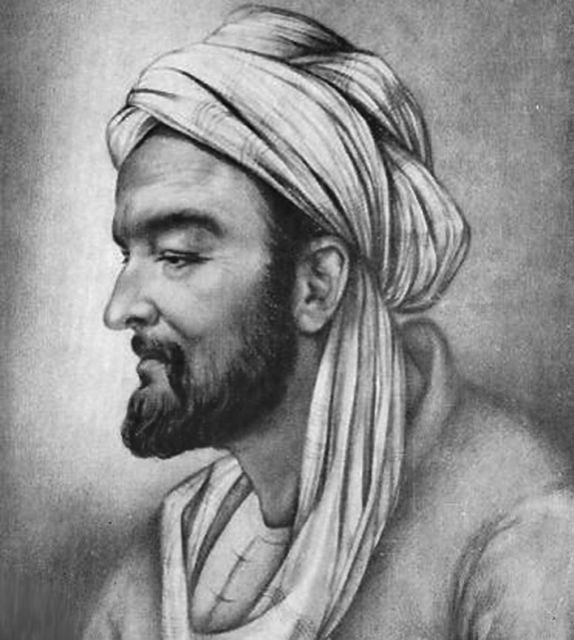
\includegraphics[width=5cm]{images/abu_ali.jpg}
  \caption{«Коль смолоду избрал к заветной правде путь,
С невеждами не спорь, советы их забудь». }
\end{marginfigure}

Каждый Мудрец может постигнуть Истину самостоятельно с вероятностью $1/9$
или же от соседа\footnote{Студенты постигают Истину примерно также!}.
Независимо от способа постижения Истины,
просветлённый Мудрец поделится Истиной с соседом слева с вероятностью $2/9$ и
с соседом справа также с вероятностью $2/9$ (независимо от соседа слева).


\begin{enumerate}
\item Какова вероятность того, что
Абу Али Хусейн ибн Абдуллах ибн аль-Хасан ибн Али ибн Сина постигнет Истину?
\item Как изменится ответ, если ряд Мудрецов бесконечен в обе стороны?
\end{enumerate}

\begin{sol}
Если $\gamma$ — вероятность самостоятельного познания Истины,
а $\alpha$ — передачи Истины отдельно в каждую из сторон, то
\[
p = \gamma + (1-\gamma) p \alpha.
\]

То есть $p=\gamma/(1-\alpha(1-\gamma))$.

Для решения второго пункта наложим на
Абу Али Хусейн ибн Абдуллах ибн аль-Хасан ибн Али ибн Сина обет молчания.
Это не повлияет на вероятность постижения им Истины,
однако превратит задачу в две уже решённых :) Получаем

\[
q = \gamma + (1-\gamma)(2p\alpha - p^2\alpha^2)
\]

\end{sol}

\end{problem}


\begin{problem}
Мост через реку Квай

Мост через реку Квай состоит из нескольких секций.
При подрыве моста каждая из секций разрушается независимо от других с вероятностью $1/2$.

\begin{tikzpicture}
\node[fill, circle, draw, blue] at (0, 0) {};
\node[fill, circle, draw, blue] at (0, 1) {};
\node[fill, circle, draw, blue] at (1, 0) {};
\node[fill, circle, draw, blue] at (1, 1) {};
\node[fill, circle, draw, blue] at (2, 0) {};
\node[fill, circle, draw, blue] at (2, 1) {};
\end{tikzpicture}

Какова вероятность того, что после подрыва моста,
по нему можно будет перебраться с одного берега на другой?
\begin{sol}
Рассмотрим двойственный граф, получаем $1/2$.
\end{sol}

\end{problem}



\begin{problem}
Академик Андрей Дмитриевич Сахаров увлечённо рубит капусту.
Капусту рубят так: сначала качан разрезают на тонкие круглые почти плоские «блины», затем полученные «блины» рубят ножом. После длительной рубки капусты в случайных направлениях Андрей Дмитриевич выбирает случайно один из полученных многоугольников капусты.

\begin{enumerate}
\item Чему равно математическое ожидание числа сторон этого многоугольника?
\item \ldots
\end{enumerate}

\todo[inline]{Оригинал статьи? вопрос про отношение площади к чему-то там?}


\begin{sol}
Если изначально кусок капусты был $n$-угольником и было сделано $r$ разрезов, то у всех поверхностей в сумме будет $n+4r$ сторон. Значит математическое ожидание числа сторон у случайно выбираемого кусочка равно $\E(X_r)=(4r+n)/(r+1)$. Эта величина стремится к $4$ независимо от от стартового $n$.
\end{sol}

\end{problem}





\begin{problem}
Летом в большом-большом городе в случайных местах открылось много киосков с мороженым. Каждый житель выбирает всегда ближайший к своему дому киоск.
Получается, что каждому киоску с мороженым соответствует обслуживаемый им участок.


Чему равно математическое ожидание числа сторон участка обслуживаемого случайным киоском?


\begin{sol}
По формуле Эйлера $f-e+v=2$, кроме того $2e=3v$. Математическое ожидание равно $\E(X_f)=2e/f=(6f-12)/f$. При большом числе киосков $f$ получаем $6$.
\end{sol}

\end{problem}





\begin{problem}
На одной из улиц в ряд стоит много уютных домиков для одиноких мудрых старцев.
Каждый день на улицу приезжает очередной одинокий мудрый старец.
Одинокий мудрый старец никогда не поселится в домике, если в соседнем домике уже кто-то живёт.
Других предпочтений у одиноких мудрых старцев нет, и они селятся по одному в случайный из подходящих домиков.

Какая доля домиков будет в среднем занята?


\begin{sol}
Обозначим $a_n$ — ожидаемое количество занятых домиков, если всего в деревне $n$ домиков. Для малых $n$: $a_0=0$, $a_1=1$, $a_2=1$, \ldots

Последовательность $a_n$ удовлетворяет рекурсивному соотношению
\[
a_n = 1 + \frac{2}{n}\sum_{i=1}^{n-2} a_i
\]

Обозначим также $s_n = \sum_{i=1}^n a_i$, тогда окажется, что

\[
\begin{cases}
a_n = 1 + \frac{2}{n}s_{n-2} \\
s_n = s_{n-1} + a_n
\end{cases}
\]

Рассмотрим производящие функции $A(x)=\sum_{i=0}^{\infty} a_i x^i$ и $S(x)=\sum_{i=0}^{\infty} s_i x^i$.

Домножаем уравнения на $x^n$ и складываем, получаем:

\[
\begin{cases}
A(x) = \frac{1}{1-x} + 2B(x) \\
S(x) = xS(x) + A(x) \\
B'(x)=xS(x)
\end{cases}
\]

Получаем одно дифференциальное уравнение
\[
(1-x)S'(x) - S(x) = \frac{1}{(1-x)^2} + 2xS(x)
\]

Из $s_0=0$ следует начальное условие $S(0)=0$. Решение уравнения имеет вид

\[
\begin{cases}
S(x)=\frac{1-e^{-2x}}{2(1-x)^3} \\
A(x)=\frac{1-e^{-2x}}{2(1-x)^2}
\end{cases}
\]

Исследуем асимптотику функции. Разложим числитель $A(x)$ в ряд Тейлора в окрестности $x=1$:
\[
A(x)= \frac{1 + e^{-2}}{2} (1-x)^{-2} + e^{-2}(1-x)^{-1} + R(x)
\]

Раскладывая в ряд Тейлора $(1-x)^{-2}$, $(1-x)^{-1}$ и $R(x)$ получаем:
\[
a_n = \frac{1-e^{-2}}{2}n + \frac{1-3e^{-2}}2 + r_n
\]

Здесь $r_n$ убывает быстро, поэтому доля занятых домиков сходится к $\frac{1-e^{-2}}{2} \approx 0.4323$.

\url{http://fivethirtyeight.com/features/can-you-solve-the-puzzle-of-your-misanthropic-neighbors/}
\end{sol}


\end{problem}



\begin{problem}
Во дворе вдоль тротуара идёт неразмеченная парковка для мотоциклов.
Общая длина парковки — $a$ метров.
Тру мотоциклисты всегда паркуются перпендикулярно тротуару.
Чтобы припарковаться одному мотоциклисту требуется один метр длины парковки. Если бы парковка была размечена и каждый мотоциклист парковался бы по разметке, то на парковку влезло бы $a$ мотоциклов. Однако парковка не размечена, а тру мотоциклисты не заморачиваются и паркуются на свободном пространстве в случайных местах, равномерно по доступной для парковке длине.

Сколько в среднем мотоциклов влезет на парковку?
\begin{sol}

\end{sol}

\end{problem}



\begin{problem}
Накануне войны Жестокий Тиран очень большой страны издал указ. Отныне за каждого новорождённого мальчика семья получает денежную премию, но если в семье рождается вторая девочка, то всю семью убивают. Бедные жители страны запуганы и остро нуждаются в деньгах, поэтому в каждой семье дети будут появляться до тех пор, пока не родится первая девочка.

\begin{enumerate}
  \item Каким будет среднее число детей в семье?
  \item Какой будет доля мальчиков в стране?
  \item Какой будет средняя доля мальчиков в случайной семье?
  \item Сколько в среднем мальчиков в случайно выбираемой семье?
\end{enumerate}

\begin{sol}
\begin{enumerate}
  \item $2$
  \item $1/2$
  \item $\sum 0.5^{i} \frac{i-1}{i} = \sum 0.5^{i}-\sum 0.5^{i}\frac{1}{i} = 1 + \ln(1/2)=1 - \ln 2$
  \item $1$
\end{enumerate}
\end{sol}

\end{problem}





\begin{problem}
Задача про Stein paradox


\begin{sol}

\end{sol}

\end{problem}


\begin{problem}
Франк Альберт Бенфорд положил на счёт в банке один доллар.
Сумма на счету растёт непрерывно с постоянной ставкой 1\% в течение длительного промежутка времени.
В случайный момент этого промежутка Франк Альберт говорит «Стоп!»

\begin{enumerate}
\item Каков закон распределения первой цифры суммы на счету?
\item А второй цифры?
\item Являются ли первая и вторая цифра независимыми случайными величинами?
\item Изменится ли ответ, если процентная ставка будет равна двум процентам?
\end{enumerate}

\begin{sol}

\end{sol}

\end{problem}


\begin{problem}
Теорема 123. Пусть $k$ — произвольное натуральное число.
Докажите, что для любых независимых одинаково распределённых $X$ и $Y$ верно неравенство:
\[
\P(|X-Y| \geq k) \leq (2k-1) \P(|X-Y| \leq 1)
\]


\begin{sol}
\url{http://www.tau.ac.il/~nogaa/PDFS/123.pdf}

Доказательство основано на детерминистическом факте.
Если есть произвольный числовой вектор $v$, и $S_k$ — это количество пар элементов вектора $v$,
отстоящих друг от друга не дальше, чем на $k$, $S_k = \card \{ (i, j) | |v_i - v_j| \leq k\}$, то $S_k < (2k-1) S_1$.

Декартово произведение $v \times v$ представляет собой сеточку точек.
Точки мы рассматриваем с учётом их кратности:

\todo[inline]{картинка}

Разделим плоскость на диагональные полосы единичной ширины. Мы докажем, что каждая полоса содержит строго меньше элементов, чем две центральных полосы в сумме. Будем добавлять элементы по одному или блоками, двигаясь змейкой вправо-вверх. При этом на центральную полосу будет добавляться либо один элемент, либо блок.


\todo[inline]{картинка}

Самый плохой случай — регулярная сетка:

\todo[inline]{картинка}

Две центральных полосы дают $S_1$ точек. Каждая полоса кроме двух центральных даёт меньше $S_1$ точек. Нецентральных полос всего $2(n-1)$ штуки. Итого точек на квадрате оказывается меньше, чем $S_1 + 2(n-1)S_1 = (2n-1) S_1$.

Переходим к вероятностной части.

Обозначим вероятность $p_k = \P(|X-Y| \geq k)$. Рассмотрим последовательность из $m$ одинаково распределённых и независимых $X_i$. Для неё выполнено доказанное детерминистическое неравенство:

\[
S_k < (2k-1) S_1
\]

Берём математическое ожидание слева и справа:
\[
\E(S_k) < (2k - 1) \E(S_1)
\]

В паре $(X_i, X_i)$ расстояние между элементами равно нулю, а в паре $(X_i, X_j)$ расстояние между элементами будет меньше $k$ с вероятностью $p_k$, значит $\E(S_k) = m + m(m-1) p_k$.

Итого,

\[
m + m(m-1) p_k < (2k-1) (m + m(m-1) p_1)
\]

Делим на $m(m-1)$ и устремляем $m$ к бесконечности, получаем $p_k \leq (2k - 1) p_1$.

\end{sol}

\end{problem}




\begin{problem}
У старухи Шапокляк счётное количество шляп. В каждую шляпу Шапокляк кладёт бумажку с произвольным рисунком по своему выбору. Гена и Чебурашка имеют право ознакомиться с содержимым практически всех шляп. Одну шляпу, какую пожелают, Гена и Чебурашка обязаны оставить закрытой. Гена и Чебурашка должны идеально точно угадать рисунок в закрытой шляпе.
\begin{enumerate}
\item Приведите пример стратегии, обеспечивающей Гене и Чебурашке вероятность выигрыша более 99\%.

\item Существует ли стратегия, обеспечивающая вероятность выигрыша более 99\%, если Гене и Чебурашке требуется угадать идеально точно бесконечное количество рисунков?
\end{enumerate}

\begin{sol}
Рассмотрим все возможные последовательности рисунков. Назовём две последовательности рисунков эквивалентными, если начиная с какого-то момента они совпадают. В каждом классе эквивалентных последовательностей выберем свою каноническую последовательность.

Гена и Чебурашка выбирают случайно натуральное число $m$ от 0 до 99 и открывают все шляпы с номерами дающими остатки от деления на 100 отличными от $m$.

Рассмотрим остаток $k\neq m$. Последовательность рисунков в шляпах дающих $k$ в остатке эквивалентна некоторой канонической последовательности рисунков. Совпадение с канонической начинается с некоторого номера $n_k$. Выберем максимальное из $n_k$, $n=\max_{k\neq m} n_k$

В рамках подпоследовательности шляп дающих $m$ в остатке откроем все шляпы с номерами $n + 2$, $n + 3$, \ldots. По этим картинкам поймём каноническую последовательность.

Выскажем догадку, что в подпоследовательности шляп дающих $m$ в остатке на месте $n+1$ находится каноническая картинка.

Гена и Чебурашка проиграют, только если выбрали $m$ при котором совпадение подпоследовательности с канонической начинается позже всего. А вероятность этого не превосходит одну сотую.
\end{sol}

\end{problem}




\begin{problem}
Wilmott, оптимальная остановка для числа черных минус число красных карт -> тут только динопт?
\begin{sol}

\end{sol}

\end{problem}



\begin{problem}
У домашнего учителя Алексея Ивановича один фридрихсдор. Перед ним обычная колода в 52 карты.
Перед открытием каждой карты Алексей Иванович выбирает, какую долю своего богатства,
от нуля до единицы, поставить на цвет следующей карты. Карты бывают двух цветов: чёрные и красные.
Например, у Алексея Ивановича есть такая стратегия:
не ставить ничего вплоть до последней карты и затем поставить весь рубль на нужный цвет.
Такая стратегия гарантированно удвоит его богатство.

Найдите стратегию, которая максимизирует гарантированный выигрыш Алексея Ивановича.
Чему равен этот максимальный гарантированный выигрыш?
\begin{sol}

\end{sol}

\end{problem}


\begin{problem}
От станции Ромашково друг за другом в одном направлении отходит 100 паровозиков с интервалом в одну минуту. Стартовые скорости паровозиков — независимые, равномерные на $[0;1]$ случайные величины. Когда более быстрый паровозик догоняет более медленный, он снижает свою скорость до скорости догнанного паровозика.

Через достаточно длинный интервал времени паровозики разобьются на несколько групп.

\begin{enumerate}
  \item Какова вероятность того, что пятый паровозик — лидер очередной группы?
  \item На сколько групп в среднем разбиваются паровозики?
  \item Зависимы ли события: третий паровозик — лидер группы и пятый паровозик — лидер группы?
  \item Чему равна дисперсия количества групп?
\end{enumerate}


\begin{sol}
Рассмотрим, скажем, третий паровозик. Он начнёт рано или поздно новую группу, если и только если стартовал медленнее каждого из первых двух. Иначе он рано или поздно догонит более медленного. Значит, вероятность того, что третий является лидером группы равна $1/3$.

Разбиваем искомую величину $N$ в сумму индикаторов, $N=X_1 + X_2 + \ldots + X_n$ и получаем:
\[
\E(N) = 1 + \frac{1}{2} + \frac{1}{3} + \ldots + \frac{1}{n}.
\]
События «третий паровозик — лидер группы» и «пятый паровозик — лидер группы» независимы. Действительно, если пятый паровозик — лидер, то это означает, что он движется медленнее первых четырёх, но ничего не говорит о порядке этих самых четырёх.

Стало быть, дисперсия разбивается в сумму:
\[
\Var(N) = 0 + \frac{1}{2}\left(1 - \frac{1}{2}\right) + \frac{1}{3}\left(1 - \frac{1}{3}\right) + \ldots + \frac{1}{n}\left(1 - \frac{1}{n}\right)
\]
\end{sol}
\end{problem}


\begin{problem}

\todo[inline]{Тут график с обозначенным началом, концом, мин и макс.}

Начинающий трейдер Афанасий совершает не более одной сделки в день.

Если в какой-то день у трейдера Афанасия есть акция,
то за этот день он равновероятно продаёт или не продаёт её.
Если в какой-то день у трейдера Афанасия нет акций,
то он равновероятно покупает или не покупает одну акцию.

Найдите ожидаемую прибыль Афанасия.
\begin{sol}

\end{sol}
\end{problem}


\begin{problem}
  \todo[inline]{Проверить про нечётность!}
  В мешке 100 монеток. Из них 37 правильных. Все 100 монеток подбрасывают одновременно.

  Какова вероятность того, что выпадет чётное количество орлов?
\begin{sol}

\end{sol}
\end{problem}

\begin{problem} Задача о 100 заключённых и лампочке

У ста узников тюрьмы есть последний шанс на спасение.
Узники сидят в одиночных камерах и не могут общаться между собой.
Каждый день начальник тюрьмы выбирает одного заключенного наугад и
приводит в особую комнату с лампочкой. Каждый заключённый может свободно включать и выключать лампочку.
Затем начальник возвращает заключённого обратно в камеру.

Во время посещения особой комнаты заключённый имеет право сказать «Все посетили особую комнату».
Если он прав, то всех освобождают, если нет — то всех убивают.

Заключённые могут заранее договориться об используемой стратегии.

  \begin{enumerate}
    \item Заключённые предложили стратегию: подождать 5 лет,
    а потом первый заходящий в комнату говорит, что её уже все посетили.
    Какова вероятность спасения при использовании такой стратегии?
    \item Укажите стратегию, которая гарантирует заключённым спасение с вероятностью равной единице.
    Постарайтесь подобрать стратегию так, чтобы ожидаемое время спасения было наименьшим.
    За какое время в среднем данная стратегия завершается?
  \end{enumerate}

\begin{sol}
Одна из возможных стратегий: выбрать среди заключённых капитана.
Каждый заключённый кроме капитана ведёт себя так: увидев включённую лампочку ничего не делает,
увидев выключенную в первый раз — включает её, а все последующие выключенные не трогает.
Капитан всегда выключает лампочку, если это возможно. Если капитан выключил лампочку 100 раз,
значит все 99 остальных уже включили её по разу.
\end{sol}
\end{problem}


\begin{problem}
В стиральной машинке перемешались во время стирки $n$ разных пар носков. Число $n$ достаточно велико.
\begin{enumerate}
  \item Я в случайном порядке достаю носки по одному до получения первой пары. Пусть мне потребуется $T$ носков. Найдите точное значение $\E(T)$, примерное выражение для $\E(T)$ без факториалов и примерное значение $\P(T/\sqrt{n} \leq x)$.
  \item Я достаю случайное количество носков $S$, где $S$ равновероятно от 0 до $2n$ включительно. Сколько в среднем полных пар я достану?
\end{enumerate}

\begin{sol}
$2^{2n}/C_{2n}^n$, $\sqrt{\pi n}$, $1-\exp(x^2/4)$; $N/3$
\autocite{friedlen1990e3265}, \autocite{894509}
\end{sol}
\end{problem}

\begin{problem}
К продавцу мороженого выстроилась очередь.
Продавец узнает у каждого день рождения. При первом совпадении дня рождения он дарит мороженое бесплатно.
\begin{enumerate}
\item При какой длине очереди вероятность наличия счастливчика впервые становится больше $0.5$? \item Каким нужно встать в очередь, чтобы максимизировать шансы на бесплатное мороженое?
\item Чему при этом будет равна вероятность получения бесплатного мороженого?
\end{enumerate}

\begin{sol}
Обозначим вероятность бесплатного мороженого как $p_n$.
Условие $p_n > p_{n+1}$ равносильно тому, что $n^2 - n >365$. Решаем неравенство и получаем $n > \sqrt{365.25} + 0.5 \approx 19.1$. Поэтому лучше всего стоять 20-м. Вероятность бесплатного мороженого примерно равна $0.03$.
\end{sol}
\end{problem}


\begin{problem}
У Саши и Маши по колоде карт.
Они тасуют свои колоды и начинают синхронно открывать карты по одной.
Какова вероятность того, что их карты ни разу не совпадут?
\begin{sol}
Достаточно тасовать одну колоду. Получаем $1/e$.
\end{sol}
\end{problem}


\begin{problem}
Рассмотрим треугольник $\Delta ABC$.
Высота проведённая к стороне $AB$ известна и равна $h_C$.
Внутри треугольника случайно равномерно выбирается точка $X$.

Чему равно ожидаемое расстояние от точки $X$ до прямой $AB$?
\begin{sol}
Для удобства расположим сторону $AB$ горизонтально. Если $D$ — центр масс треугольника (вектор математических ожиданий двух координат), то
\[
\vec{CX} = \frac{\vec{CA} + \vec{CB}}{3}.
\]
Доказать это можно разрезав треугольник на четыре равных треугольника. Данное равенство можно разложить на вертикальную и горизонтальную составляющую. Вертикальная составляющая у $\vec{CA}$ и $\vec{CB}$ одинаковая. Следовательно, ожидаемая вертикальная составляющая от $C$ до $X$ равна $2/3$ высоты, а искомое математическое ожидание равно $h_C/3$.

Можно, конечно, и интеграл взять, но это не так элегантно :)

Альтернативное решение без интегралов. Ожидаемое расстояние линейно зависит от высоты. Осталось только найти коэффициент. Найдём ожидаемую сумму трёх расстояний до прямых.

Расстояние до прямой — это линейная функция от координат точки $(x, y)$. Значит сумма трёх расстояний тоже линейная функция. Следовательно (нужно подробнее), ожидание суммы равно среднему арифметическому расстоянию в вершинах треугольника. То есть ожидание суммы трёх расстояний равно среднему суммы трёх высот. Мы нашли, что искомый коэффициент равен одной трети.
\end{sol}
\end{problem}


\begin{problem}
У Винни-Пуха опилки в голове, поэтому запомнить больше двух натуральных чисел Винни-Пух не в состоянии.
Кролик будет называть вслух по одному некоторые натуральные числа и в заранее неизвестный момент скажет «Стоп!»
Винни-Пух точно знает, что одно из натуральных чисел — любимое число Кролика,
поэтому Кролик назовёт это число более чем в половине случаев.

Как Винни-Пуху определить любимое число Кролика?
\begin{sol}
  Достаточно помнить число-лидер и на сколько оно опережает всех конкурентов вместе взятых.
\end{sol}
\end{problem}


\begin{problem}
Ёжик и Медвежонок каждый вечер считают звёзды, и соревнуются, кто насчитает больше.
Ёжик и Медвежонок одинаково внимательны, поэтому вероятность победы Ёжика равна $1/2$.

\begin{enumerate}
  \item Какова вероятность того, что наступит такой день, в который окажется, что Ёжик выиграл в два раза больше вечеров, чем Медвежонок?

  \item Как изменится ответ, если вероятность победы Ёжика в отдельный вечер равна $p$?
\end{enumerate}
  \begin{sol}
    \url{https://math.stackexchange.com/questions/60021}
  \end{sol}
\end{problem}

\begin{problem}
  \url{https://artofproblemsolving.com/community/c7t193f7h1579002_breaking_a_stick_at_n1_points_to_form_a_convex_ngon}
  \begin{sol}
  \end{sol}
\end{problem}

\begin{problem}
  \url{https://artofproblemsolving.com/community/c7t193f7h1557638_probability_that_a_positive_integer_is_squarefree}
  \begin{sol}
  \end{sol}
\end{problem}



\begin{problem}
Примирение невозможно, и потому Андрей и Борис решаются на дуэль.
Они встают на расстоянии 40 друг от друга и начинают сходиться к барьерам.
Расстояние между барьерами 20 шагов, от дуэлянтов до барьеров изначально 10 шагов.

Вероятность промаха Бориса составляет $f_B(x)=x/40$, для Андрея — $f_A(x)=(x/40)^2$,
где $x$ — расстояние между дуэлянтами.

Как выглядит оптимальная стратегия каждого дуэлянта?

\url{https://ru.wikisource.org/wiki/Дуэльный_кодекс_В._Дурасова#Дуэль_с_приближением}
\url{https://ru.wikipedia.org/wiki/Четверная_дуэль}

\todo[inline]{непрерывность? заменить на вариант без барьеров?}

  \begin{sol}
    В равновесии в чистых стратегиях оба стреляют одновременно.
    Иначе тому, кто задумал выстрелить раньше имеет смысл подождать
    и увеличить вероятность попадания.
  \end{sol}
\end{problem}


\begin{problem}
  Ты приехал в уездный город Энск. В городе кроме тебя живут $m$ мирных граждан и $u$ убийц.
  Каждый день на улице случайным образом встречаются два человека.
  Если встречаются два мирных гражданина, то они пожимают друг другу руки.
  Если встречаются мирный гражданин и убийца, то убийца убивает мирного гражданина.
  Если встречаются двое убийц, то оба погибают.

  Каковы твои шансы выжить в этом городе, зависят ли они от стратегии поведения?
  \begin{sol}
    Если убийц нечетное число, то в живых останется только один убийца.
    Если убийц чётное число, то в живых либо не останется никого, либо мирные граждане.

    Следовательно, если кроме гостя в городе нечётное число убийц $u$, то шансов у гостя никаких нет.
    Если гость мирный, то в живых останется в финале один из убийц, если гость — убийца, то в финале убийц не останется.

    Если кроме гостя в городе чётное число убийц $u$, и гость будет новым нечётным убийцей, то в финале останется один убийца, и вероятность
    выжить для гостя равна $1/(u+1)$.

    Рассмотрим случай чётного числа убийц и мирного гостя.
    Замечаем, что прочие мирные лишь отдаляют по времени разборки и не влияют на вероятность выжить гостя.
    Поэтому уберём остальных мирных жителей.

    Чтобы гость выжил, все встречи должны быть между убийцами. Следовательно, вероятность выжить равна:

    \[
    \frac{u}{u-1}\frac{u-1}{u-2} \cdot \frac{u-2}{u-3}\frac{u-3}{u-4}\cdot \ldots \cdot \frac{2}{3}\frac{1}{2} = \frac{1}{u+1}
    \]

    От стратегии гостя ничего не зависит :)
    И вероятность выжить гостя либо 0, либо $1/(u+1)$ в зависимости от чётности числа убийц.

  \end{sol}
\end{problem}




\begin{problem}
Али-Баба хочет проникнуть в пещеру с сокровищами.
Вход в пещеру закрыт и его охраняет Джин с квадратным подносом.

В каждой вершине подноса — непрозрачный стаканчик.
Под каждым стаканчиком — монетка.

Если все четыре монетки окажутся в одинаковом положении, все — орлом вверх,
или все — решкой вверх, то вход откроется.

За одно действие Али-Баба может открыть любые два стаканчика
и положить открывшиеся монетки любой стороной вверх.

После действия Али-Бабы Джин накрывает монетки стаканчиками,
быстро-быстро вращает поднос и снова предоставляет поднос Али-Бабе.

Углядеть за Джином или сделать пометки на подносе невозможно.

\begin{enumerate}
  \item Как надо действовать Али-Бабе,
   чтобы гарантировать себе вход в пещеру за наименьшее количество действий?
   Сколько действий потребуется в худшем случае?
   \item Сколько в среднем действий потребуется Али-Бабе,
   если он просто будет выбирать два случайных стаканчика и переворачивать монетки
   орлом вверх, а изначально две монетки лежат решкой вверх, а две — орлом?
   \item Каково минимальное количество стаканчиков,
   которые Али-Бабе нужно открывать за одно действие,
   чтобы гарантированно войти в пещеру,
   охраняемую Джином с $n$-угольным подносом?
\end{enumerate}


Источник: Кордемский, Математика изучает случайности

  \begin{sol}

  \end{sol}
\end{problem}



\begin{problem}
Пират Джо вытягивает карты по одной из хорошо перемешанной колоды в 52 карты.
\begin{enumerate}
  \item На каком месте в среднем появляется первая дама?
  \item Какова вероятность того, что за первой дамой сразу появится туз пик?
  \item Какова вероятность того, что за первой дамой сразу появится дама пик?
\end{enumerate}
\begin{sol}
Возьмём колоду, добавим в неё джокера. Разложим в открытую по окружности.
Джокер означает место разрыва окружности для её выкладывания в обычную колоду.
Замечаем, что джокер и четыре дамы разбивают окружность на пять случайных отрезко.
В силу симметрии ожидаемые длины этих отрезков равны и равны по $48/5$.
Значит первая дама попадается в среднем на $48/5 + 1$ месте.

Представим, что перед разрезанием по джокеру мы переложим джокера и первого туза
в колоде разложенной по окружности. А потом разрежем окружность в стандартную
колоду по джокеру. Таким образом вопрос свёлся к тому, какова вероятность того,
что первой картой идёт туз пик или дама пик. Эти вероятности равны по $1/52$.

На первый взгляд кажется, что если шансы на туза пик равны $1/52$, то шансы на
даму пик за первой дамой меньше, так как первая дама уже могла дамой пик.

\end{sol}
\end{problem}

\begin{comment}

\begin{problem}
Злобный Дракон поймал двух принцесс, Читу и Ниту, и посадил их в разные башни
своего замка.
Затем Злобный Дракон подбросил правильную монетку бесконечное число раз.
Все результаты чётных бросков он сообщил Чите, а все результаты нечётных — Ните.
Далее Дракон предлагает каждой из принцесс назвать номер
любого подбрасывания, результат которого ей не известен.
То есть Чита должна назвать нечётный номер, а Нита — чётный.

Если результаты бросков, названных Читой и Нитой, одинаковые, то Злобный Дракон
дарит каждой принцессе тортик, плюшевого зайца и отпускает на свободу.
Если же результаты бросков отличаются, то Злобный Дракон съедает Читу и Ниту.

Принцессы знают о повадках Злобного Дракона и могли заранее до похищения договориться
о стратегиях.

\begin{enumerate}
\item Каковы шансы принцесс спастись, если Нита называет число первой,
а Чита называет своё число, зная что выбрала Нита?
\item Каковы шансы принцесс спастись, если Чита и Нита после похищения
лишены возможности передавать информацию друг другу?
\end{enumerate}

\begin{sol}

\end{sol}
\end{problem}
\end{comment}



красивые задачи из старой версии задачника\ldots


\Closesolutionfile{solution_file}

\section{Чуть менее классические задачи}

\begin{enumerate}
\item Стрелок попадает по мишени с вероятностью 0.3. Какова вероятность того, что до третьего промаха у него будет 5 выстрелов?

\item Расстояние от пункта A до B автобус проходит за 2 мин, а пешеход — за 20 мин. Интервал движения автобусов 30 мин. Вы подходите в случайный момент времени к пункту A и отправляетесь в B пешком.

\begin{enumerate}
\item Какова вероятность того, что в пути Вас догонит очередной автобус?
\item Сколько в среднем времени Вы будете добираться, если проходящий мимо автобус обязательно Вас подбирает?
\end{enumerate}

% 18/30, примерно 14 минут


\item Для простоты предположим, что ген карих глаз доминирует ген синих. Т.е. у носителя пары bb глаза синие, а у носителя пар BB и Bb — карие. У диплоидных
организмов \marginnote{А мы тут все диплоидные :)} одна аллель наследуется от папы, а одна — от мамы. В семье у кареглазых родителей два сына — кареглазый и
синеглазый. Кареглазый женился на синеглазой девушке. Какова
вероятность рождения у них синеглазого ребенка?


\item Задача о полосе невезения

За неделю Аннушка семь раз пролила масло. Какова вероятность того, что она проливала масло каждый день?



\end{enumerate}


\begin{comment}
\section{Черновые размышления :)}

сколько теории игр включать?

менее канонические задачи ??? ()




Методы: ! это отдельный документ!!!

Первый шаг

Разложение в сумму — Разделяй и властвуй

Большая сила о-малых

Матрешки — (условное математическое ожидание)

Холмс, это невероятно! (Вероятностная интерпретация)

Как сварить мартингал (теорема Дуба)

Свернулся колечком (задачи на равномерное на отрезке)


Сюжеты: ????

Пуассоновский поток

Броуновское движение



\end{comment}

\section{Решения}


% для гиперссылок на условия
% http://tex.stackexchange.com/questions/45415
\renewenvironment{solution}[1]{%
         % add some glue
         \vskip .5cm plus 2cm minus 0.1cm%
         {\bfseries \hyperlink{problem:#1}{#1.}}%
}%
{%
}%


\input{solution_file}


\listoftodos

\section{Источники мудрости}

Источники мудрости, кои автор подборки постарался не замутить.
Смело направляйте к ним верблюдов своего любопытства!

\nocite{*}

\printbibliography


\end{document}
